\documentclass{beamer}
\usepackage[utf8]{inputenc}

%\usepackage{utopia} %font utopia imported


\usepackage[official]{eurosym}
\usepackage{fancyhdr}
\usepackage{mathrsfs}
\usepackage{wrapfig}
\usepackage{setspace}
\usepackage{calc}
\usepackage{multicol}
\usepackage{cancel}
\usepackage[retainorgcmds]{IEEEtrantools}
\usepackage{amsmath}
\newlength{\tabcont}
\setlength{\parindent}{0.0in}
\setlength{\parskip}{0.05in}
\usepackage{empheq}
\usepackage{framed}
\usepackage[most]{tcolorbox}
\usepackage{xcolor}
\usepackage{graphicx}
\usepackage{graphics}
\usepackage{pgfplots}
\colorlet{shadecolor}{orange!15}
\newcommand{\bF}{\bar{F}}
\pgfmathdeclarefunction{gauss}{2}{\pgfmathparse{1/(#2*sqrt(2*pi))*exp(-((x-#1)^2)/(2*#2^2))}}
%Different Sets
\newcommand{\DD}{\mathcal D}
\newcommand{\CC}{\mathbb C}
\newcommand{\NN}{\mathbb N}
\newcommand{\FF}{\mathbb F}
\newcommand{\QQ}{\mathbb Q}
\newcommand{\RR}{\mathbb R}
\newcommand{\ZZ}{\mathbb Z}
% Theorems, equations, lemmas
\newcommand{\thm}[2]{\begin{theorem} \begin{shaded} #1 \end{shaded}\end{theorem} \begin{proof} #2 \end{proof}}
\newcommand{\eq}[1]{\begin{equation*} #1\end{equation*}}
\newcommand{\eqq}[1]{\begin{equation} #1\end{equation}}
\newcommand{\lem}[1]{\begin{lemma} #1 \end{lemma}}
\newcommand{\defin}[1]{\begin{defn} #1 \end{defn}}
\newcommand{\D}{\frac{d}{dx}}
\newcommand{\nin}{\not\in}
\newcommand{\shade}[2]{\begin{block}{ #1} #2 \end{block}}
\newcommand{\diag}[1]{\begin{tikzpicture} #1 \end{tikzpicture}}
\newcommand{\nfr}[1]{\begin{frame} #1
\end{frame}}
% end shortcuts


\usetheme{Madrid}
\usecolortheme{default}

%------------------------------------------------------------
%This block of code defines the information to appear in the
%Title page
\title[Polynomial Methods in Combinatorics] %optional
{Polynomial Methods in Combinatorics}



\author[Conrad Crowley] % (optional)
{Conrad Crowley \\[6em] Supervisor: Marco Vitturi  }

%\logo{\includegraphics[height=1.5cm]{lion-logo.jpg}}
\date{March 2022}
%End of title page configuration block
%------------------------------------------------------------



%------------------------------------------------------------
%The next block of commands puts the table of contents at the 
%beginning of each section and highlights the current section:

\AtBeginSection[]
{
}
%-----------------------------------------------------------


\begin{document}

%The next statement creates the title page.
\frame{\titlepage}
\section{Overview}
\nfr{{What are Polynomial Methods?}
A collection of techniques in Combinatorics which use polynomials and their rigidity properties
to argue a $\dots$.
\pause

\begin{example}[Rigidity and Interpolation]
\begin{itemize}
    \item Rigidity: If $P \in \RR[X_1, \dots,X_n]$ has degree $D$ and a line $\ell$ intersects $P$ in more than $D$ points then $\ell \subset Z(P)$.
    \pause
    \item Interpolation: We can do parameter-counting arguments using the fact that $\dim \RR_{\deg \leq D} [X_1, \dots, X_n]\sim D^n$.
\end{itemize}

\end{example}
}

\nfr{{Theorems proven using polynomial methods}
We examined proofs of these theorems using the polynomial method:
\begin{itemize}
    \item Kakeya Conjecture in Finite Fields: If $A \subset \FF^n$ contains a line in every direction then $|A|  \gtrsim |\FF|^n$.
    \pause
    \item Cauchy-Davenport Theorem: $|A+B| \geq \min\{p , |A| + |B| -1\}$ where $A,B \subset \ZZ_p$ and $A+B :=\{a+b \ | \ a\in A,\ b\in B\}$. \pause
    \item Joints Problem: A collection of $N$ lines in $\RR^3$ can form at most $N^{3/2}$ joints. \pause
    \item Szemerédi-Trotter Theorem: Given $S$ points and $L$ lines, there are $\lesssim (SL)^{2/3} + S + L $ point-line incidences. (i.e. $(p, \ell) \text{ s.t. } p\in \ell$) \pause
    \item Circle Tangencies: Given a (suitably non-degenerate) collection of $N$ circles in $\RR^2$, they determine $\lesssim N^{3/2}$ tangencies.
\end{itemize}
}

\nfr{{Circle Tangencies}
\begin{theorem}
    Given a (suitably non-degenerate) collection of $N$ circles in $\RR^2$, they determine $\lesssim N^{3/2}$ tangencies.
\end{theorem}
    \begin{figure}[h]
        \centering
        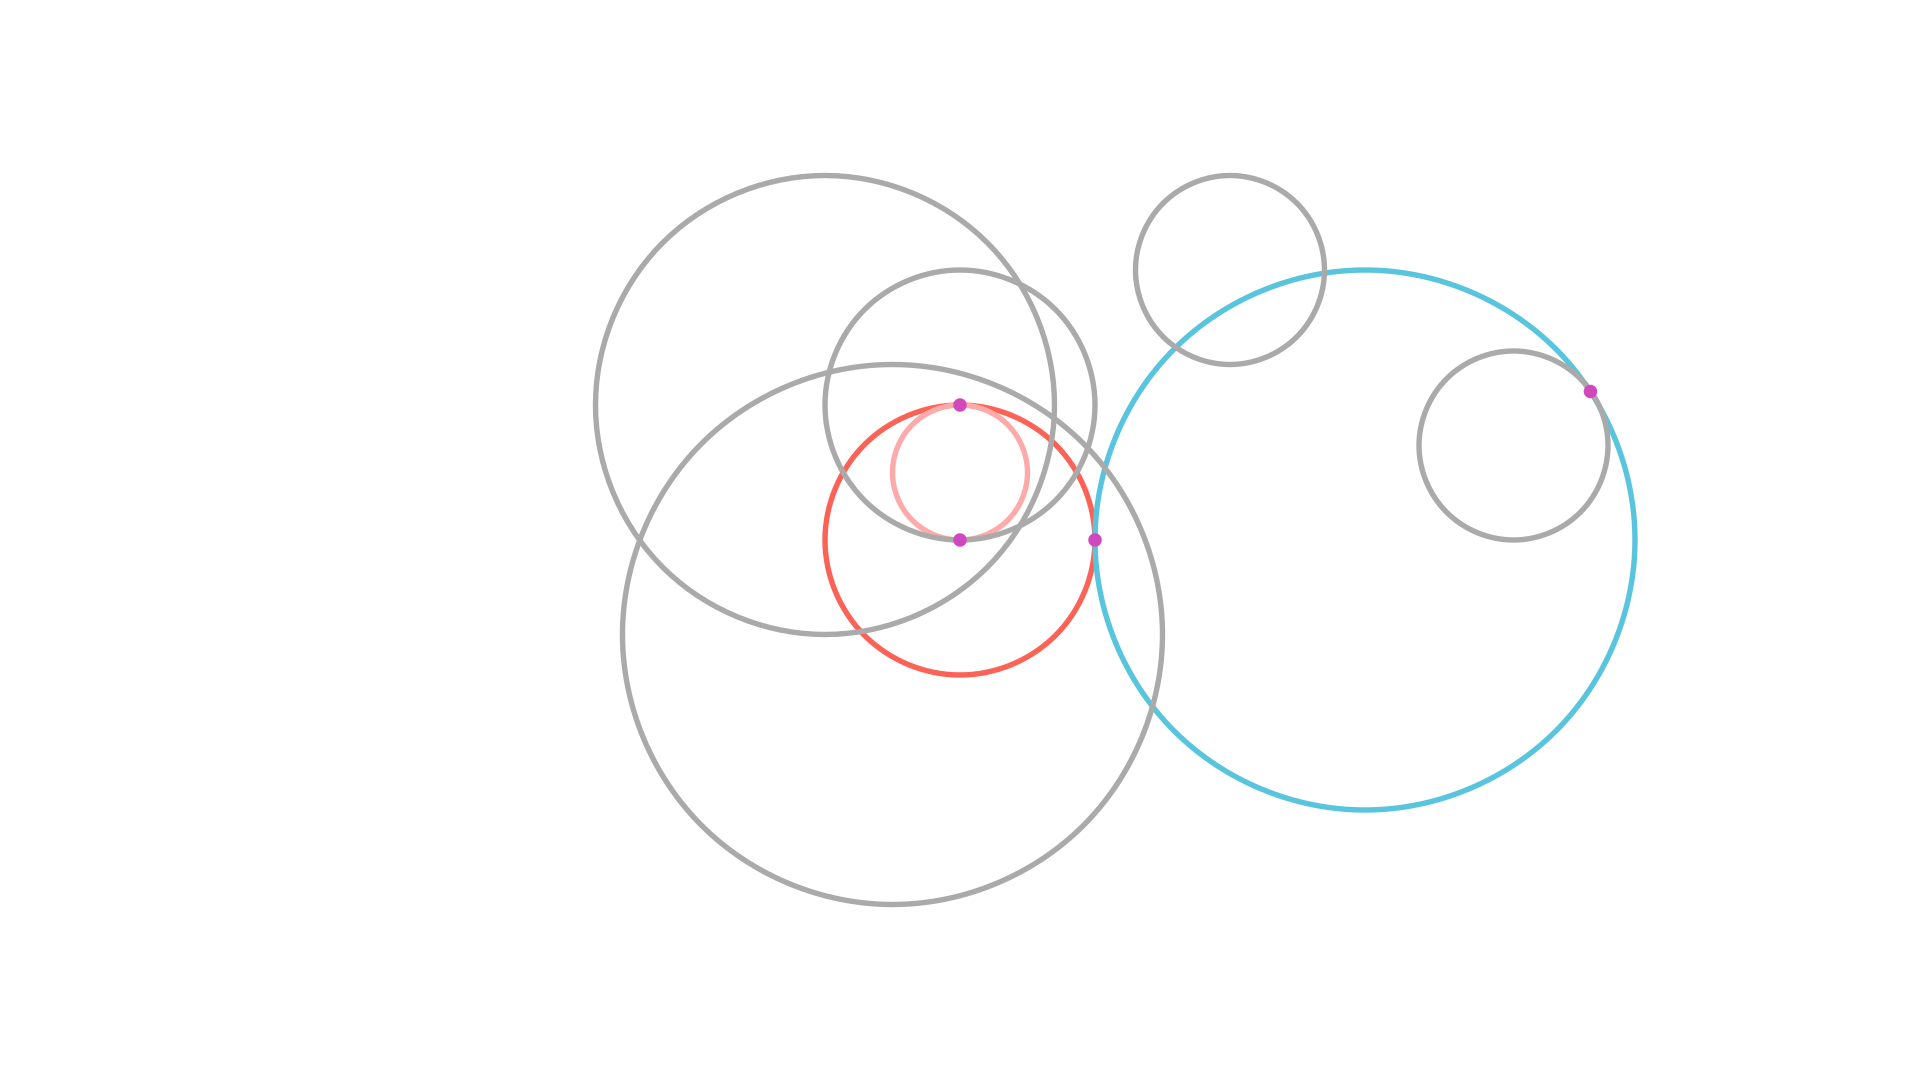
\includegraphics[trim={5cm 0 4cm 2cm}, clip,width=0.8
        \textwidth]{images/Diagram1.png}

    \end{figure}
}

\nfr{{Circle Tangencies: What's degenerate?}
\begin{figure}[h]
    \centering
    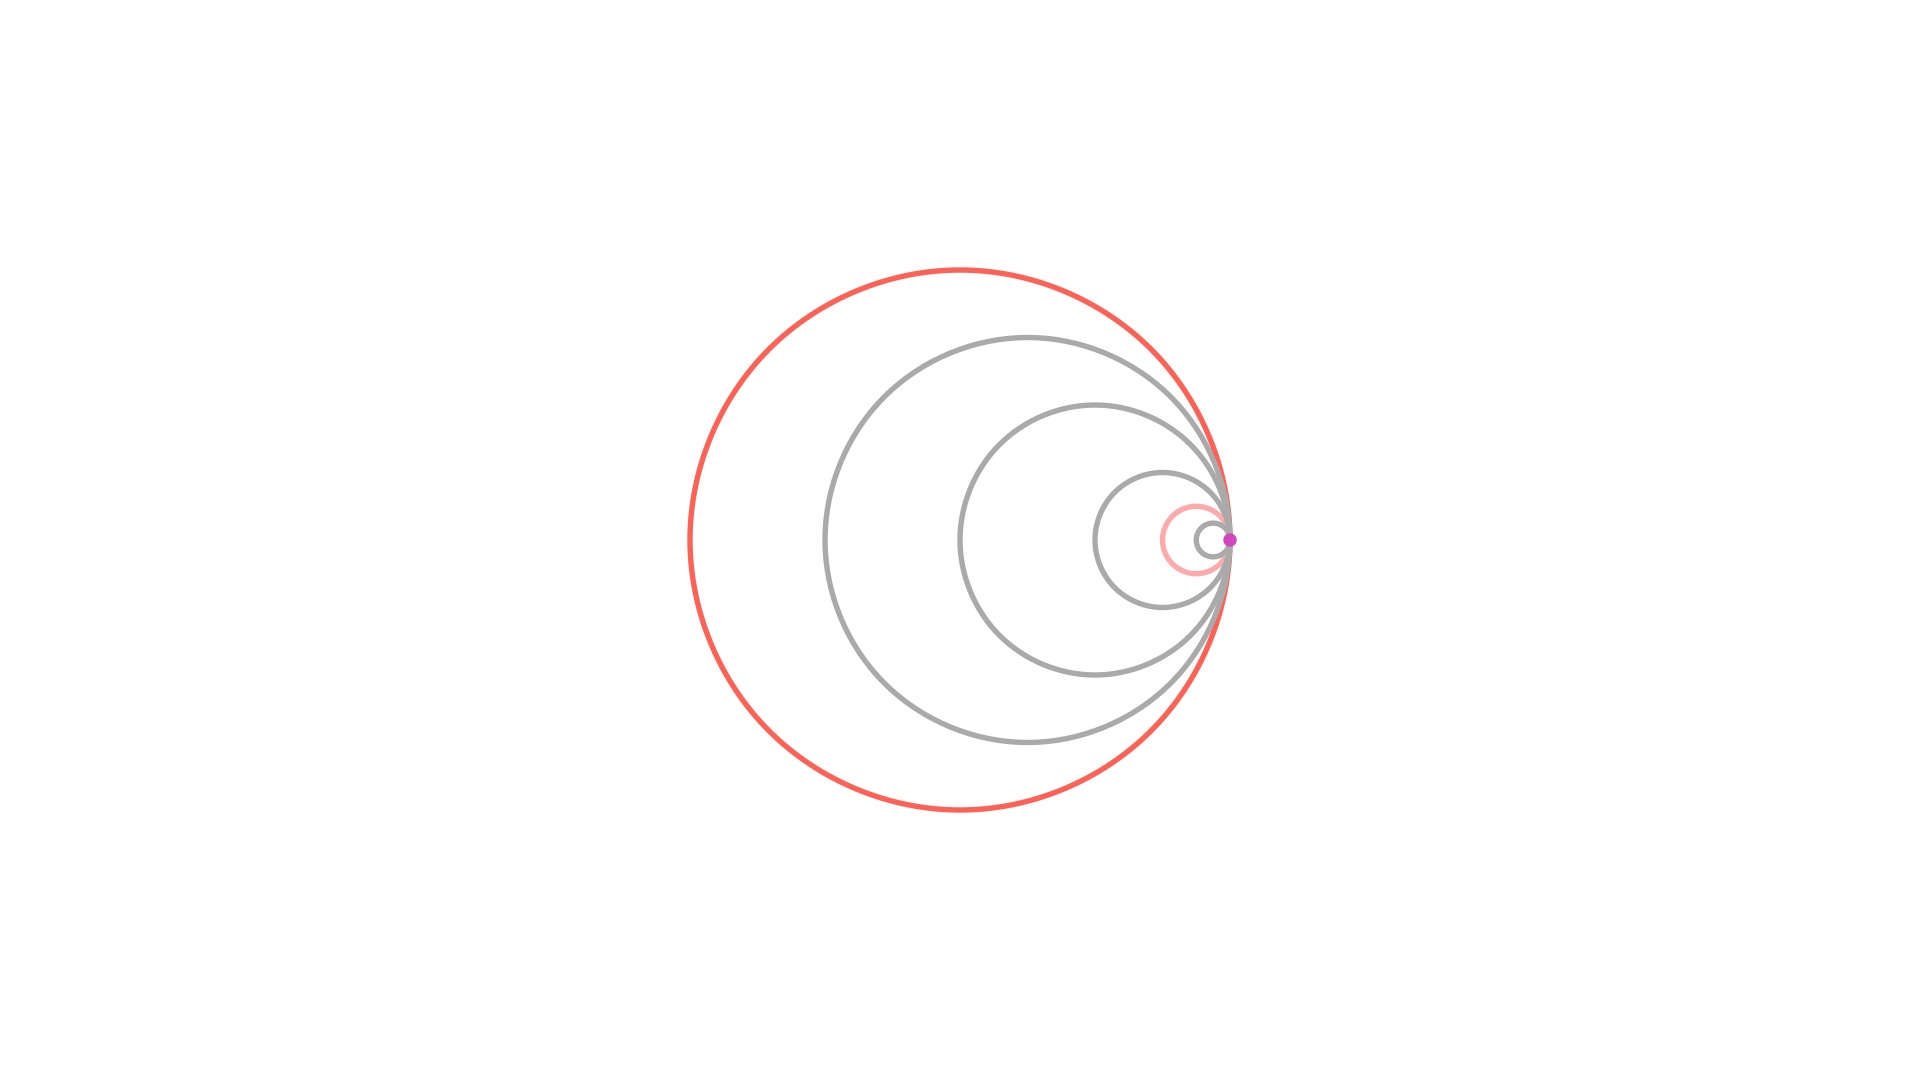
\includegraphics[width=1
    \textwidth, trim={5cm 0 4cm 2cm}, clip=true]{images/Diagram2.png}
\end{figure}
}


\nfr{{Circle Tangencies: Lifting into $\RR^3$}
\begin{theorem}
    Given a (suitably non-degenerate) collection of $N$ circles in $\RR^2$, they determine $\lesssim N^{3/2}$ tangencies.
\end{theorem}
We now present a sketch of a recent proof due to Ellenberg, Solymosi, and Zahl. \cite{ellenberg2016new}

\textbf{Sketch Proof:}
Assume that there are $\gtrsim N^{3/2}$ tangencies with each circle tangent to $\gtrsim N^{1/2}$ other circles in our collection.

For each circle $\gamma$ in our collection, we define the curve $\beta(\gamma) \subset \RR^3$ as: \[\beta(\gamma) := \left\{(x,y,z) \ | \ (x,y) \in \gamma,\ z = \frac{-1}{\text{Slope of tangent at }(x,y)} \right\}
\]


}

\nfr{{Circle Tangencies: Lifting into $\RR^3$}

\begin{figure}[h]
    \centering
    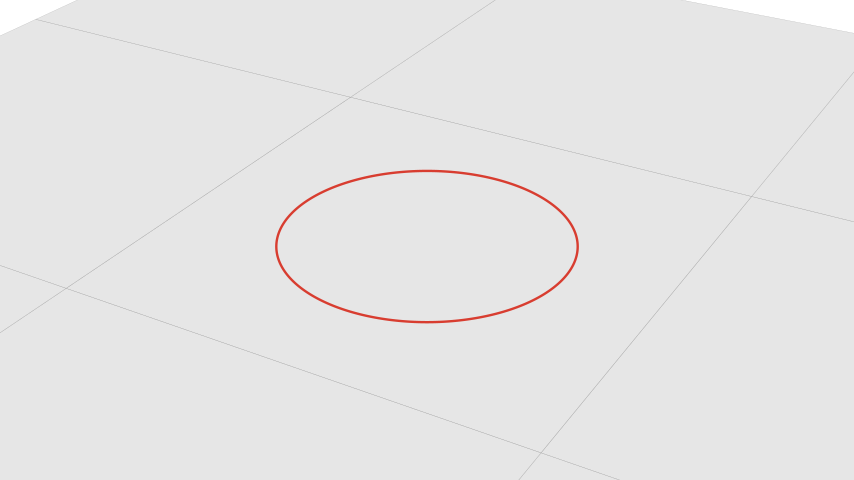
\includegraphics[width=0.8
    \textwidth, trim={5cm 0 4cm 2cm}, clip=true]{images/Diagram3a.png}
\end{figure}
}


\nfr{{Circle Tangencies: Lifting into $\RR^3$}

\begin{figure}[h]
    \centering
    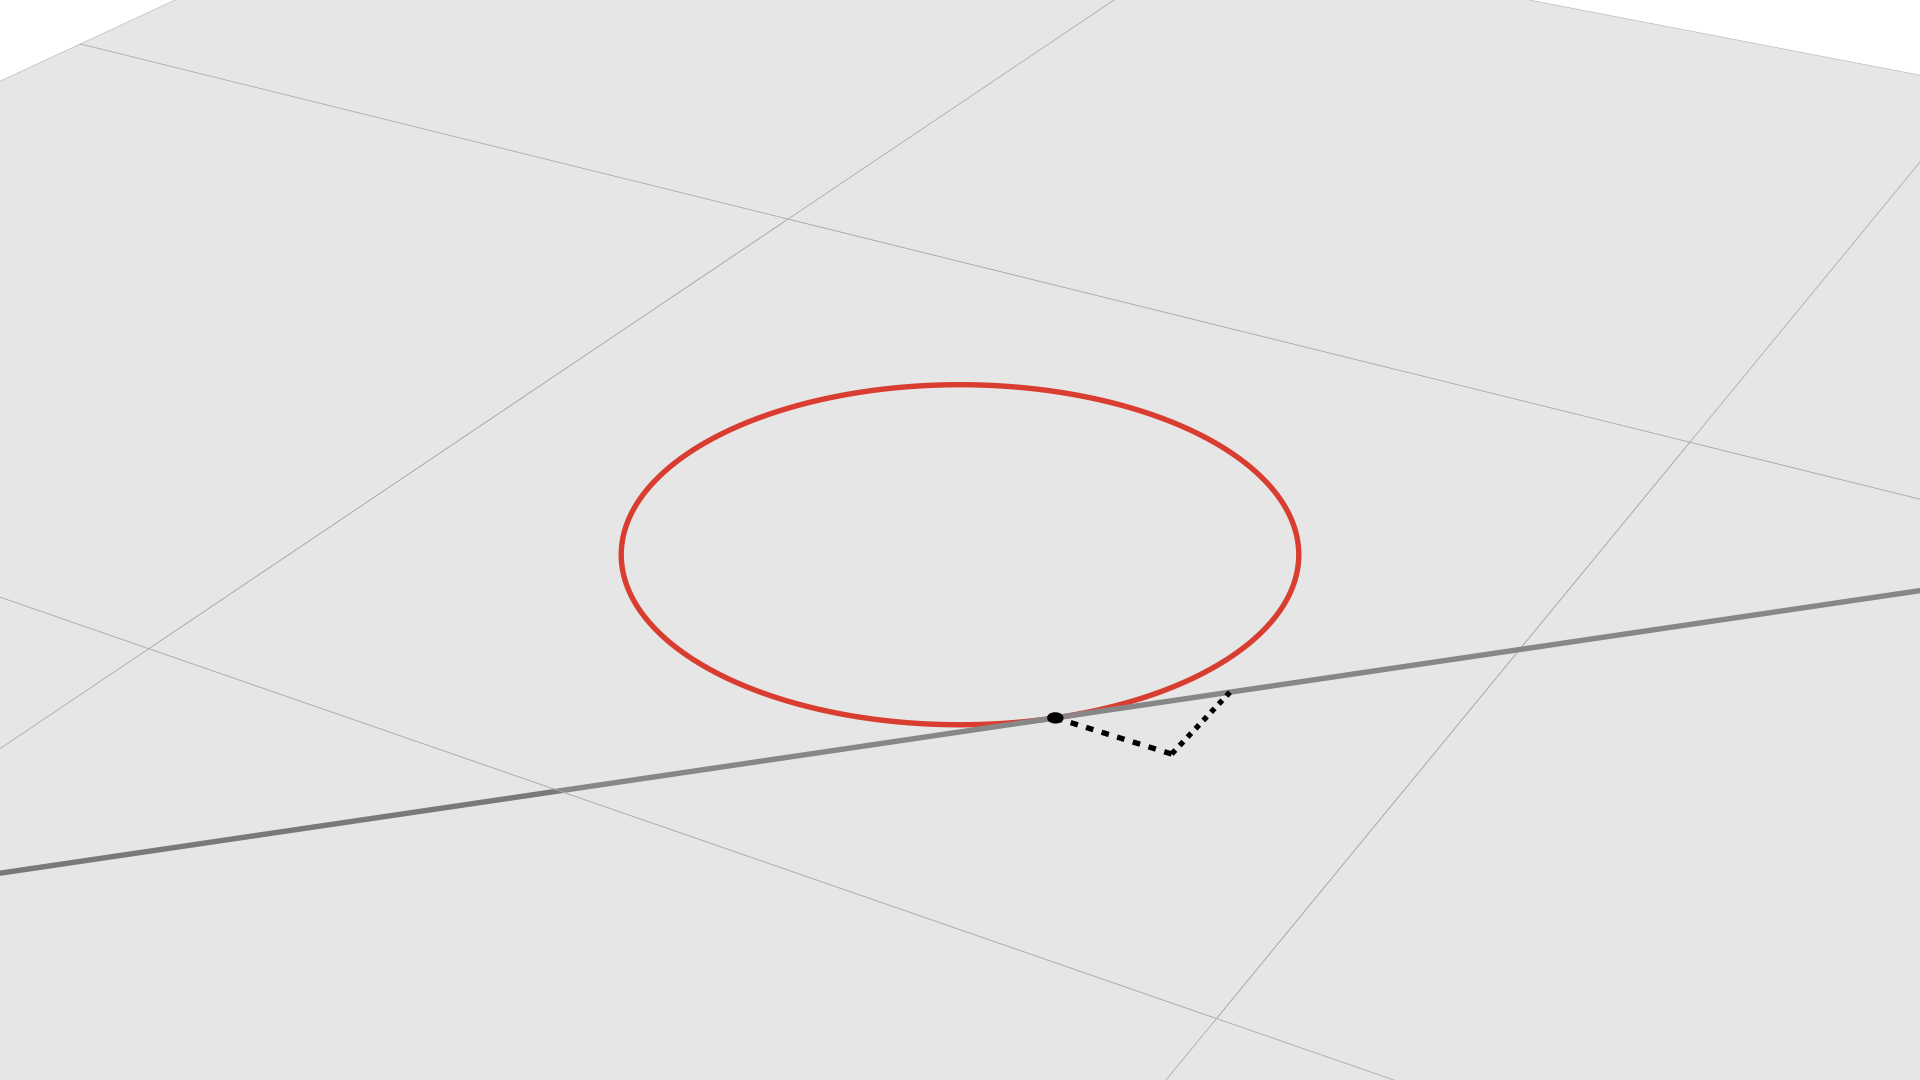
\includegraphics[width=0.8
    \textwidth, trim={5cm 0 4cm 2cm}, clip=true]{images/Diagram3b.png}
\end{figure}

}
\nfr{{Circle Tangencies: Lifting into $\RR^3$}

\begin{figure}[h]
    \centering
    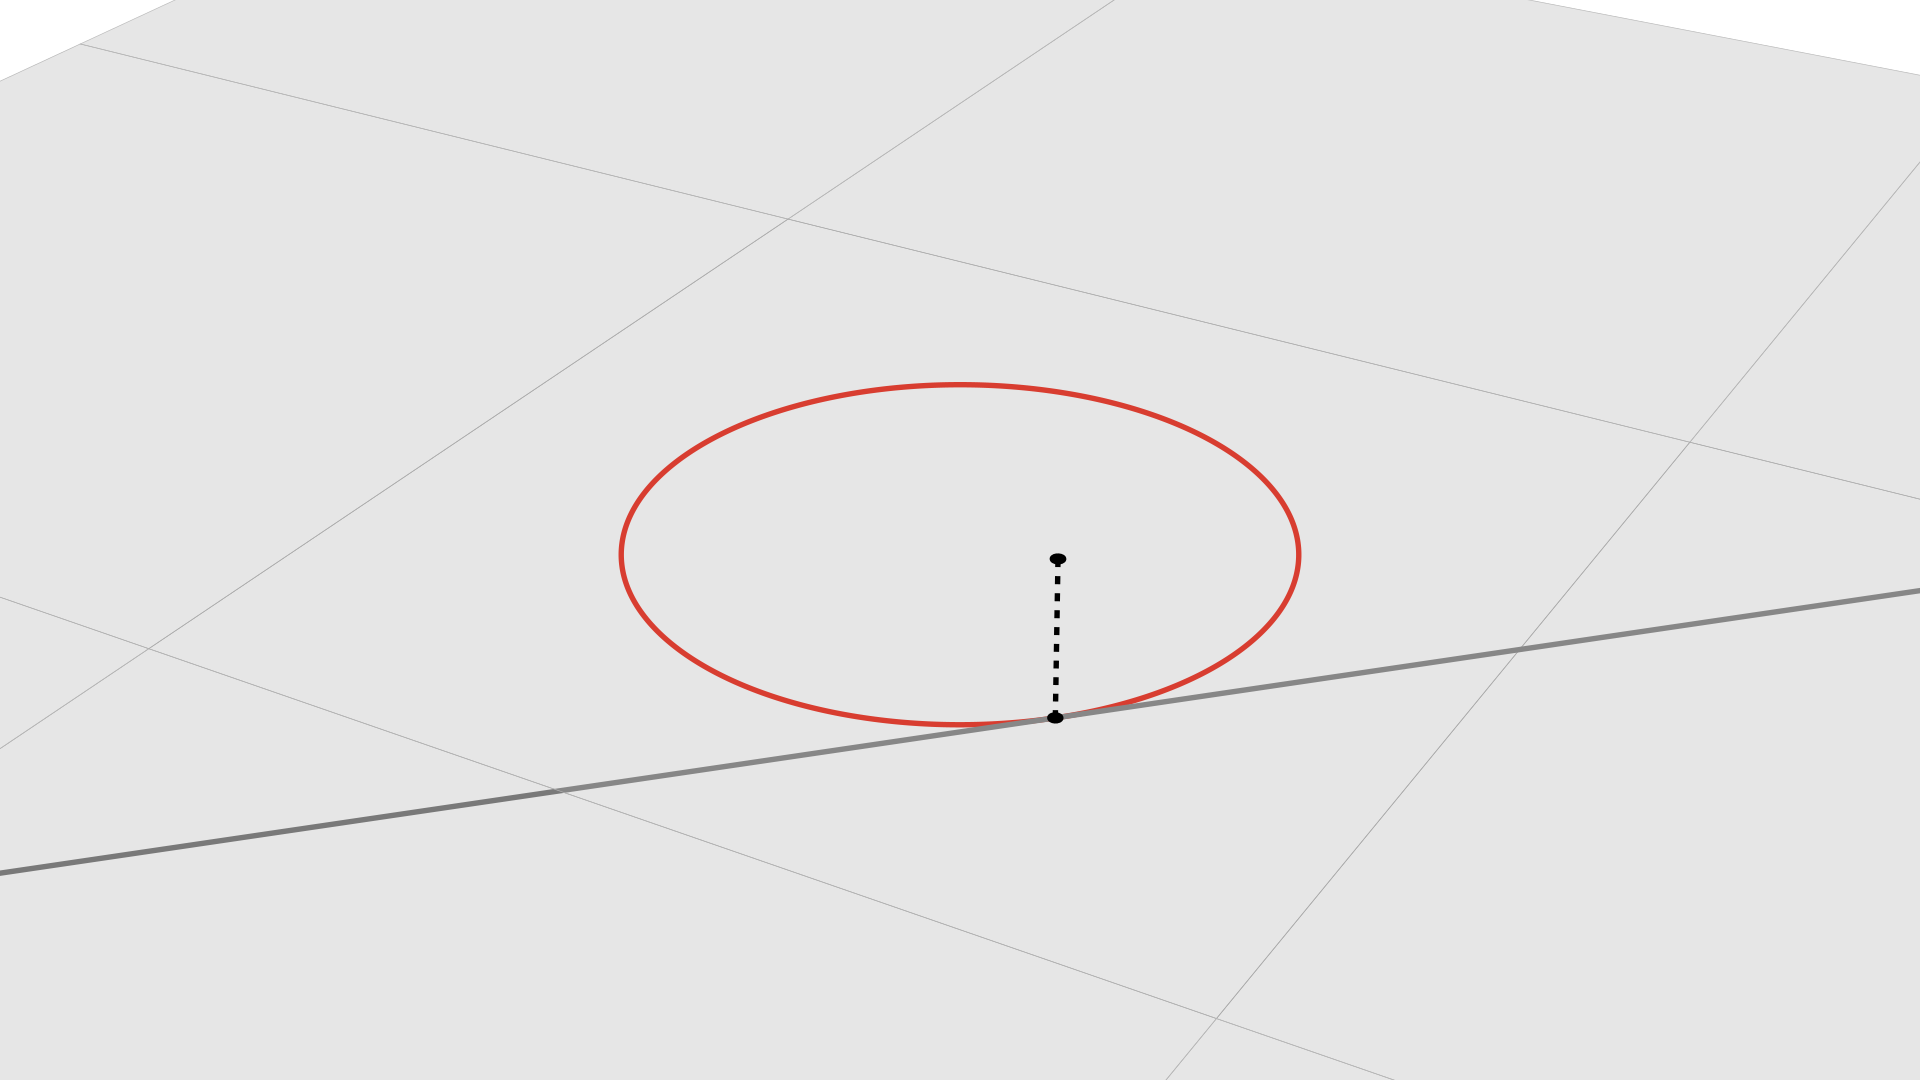
\includegraphics[width=0.8
    \textwidth, trim={5cm 0 4cm 2cm}, clip=true]{images/Diagram3c.png}
\end{figure}

}
\nfr{{Circle Tangencies: Lifting into $\RR^3$}

\begin{figure}[h]
    \centering
    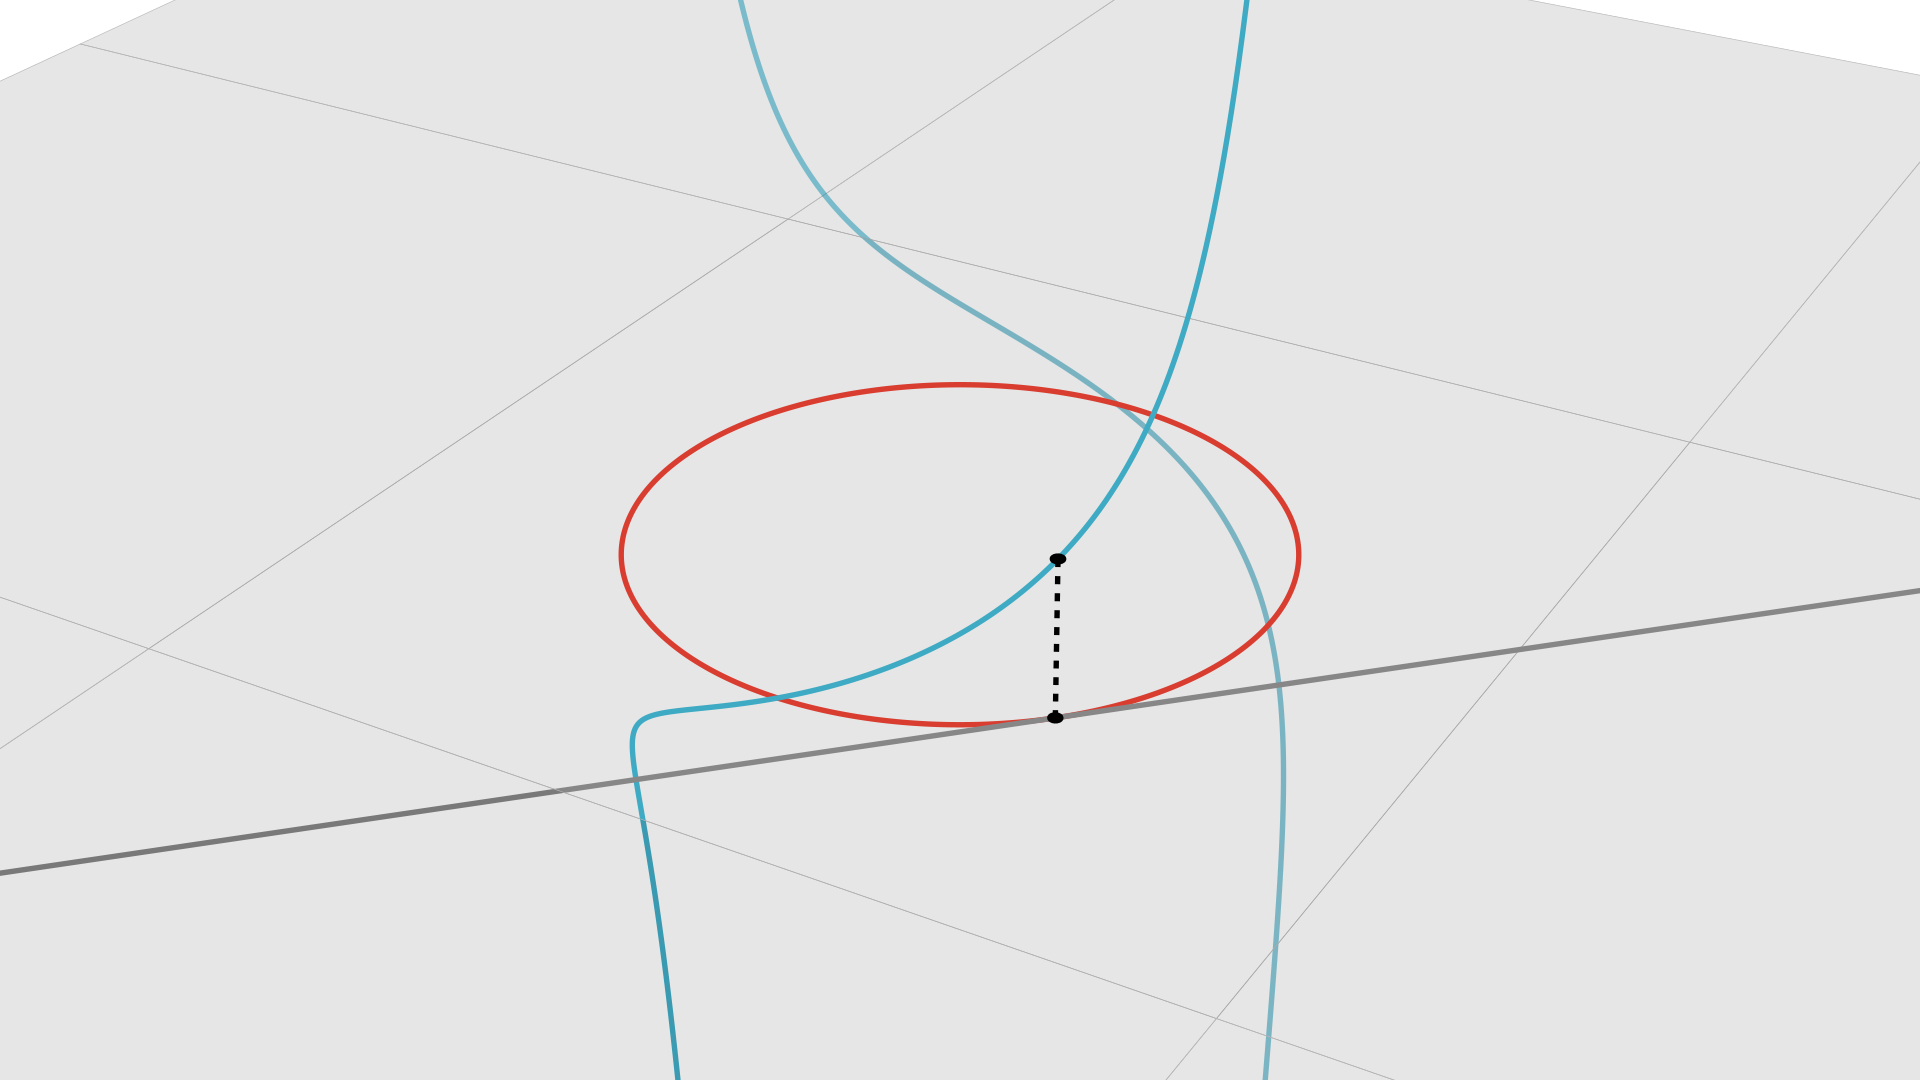
\includegraphics[width=0.8
    \textwidth, trim={5cm 0 4cm 2cm}, clip=true]{images/Diagram3d.png}
\end{figure}

}




\nfr{{Circle Tangencies: Tangencies to Incidences}

\begin{figure}[h]
    \centering
    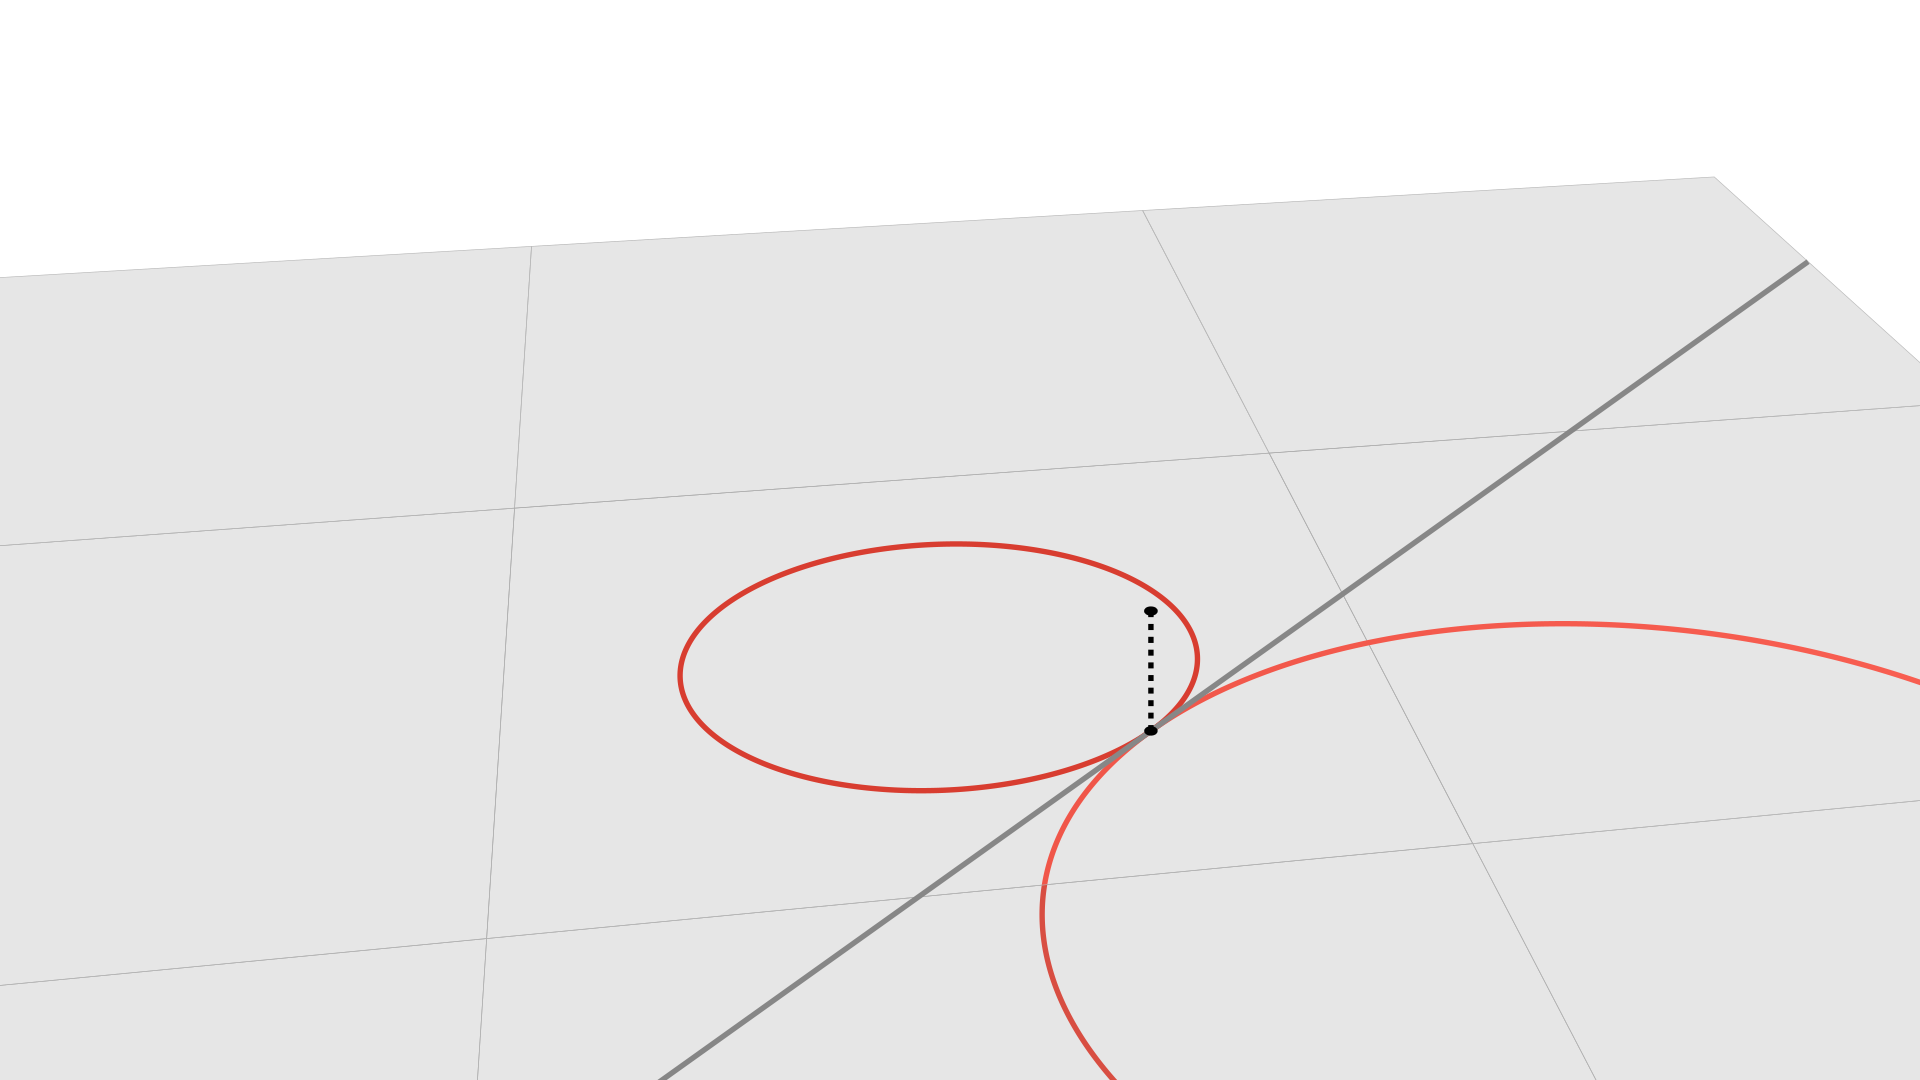
\includegraphics[width=0.8
    \textwidth, trim={5cm 0 4cm 2cm}, clip=true]{images/Diagram4a.png}
\end{figure}


}

\nfr{{Circle Tangencies: Tangencies to Incidences}

\begin{figure}[h]
    \centering
    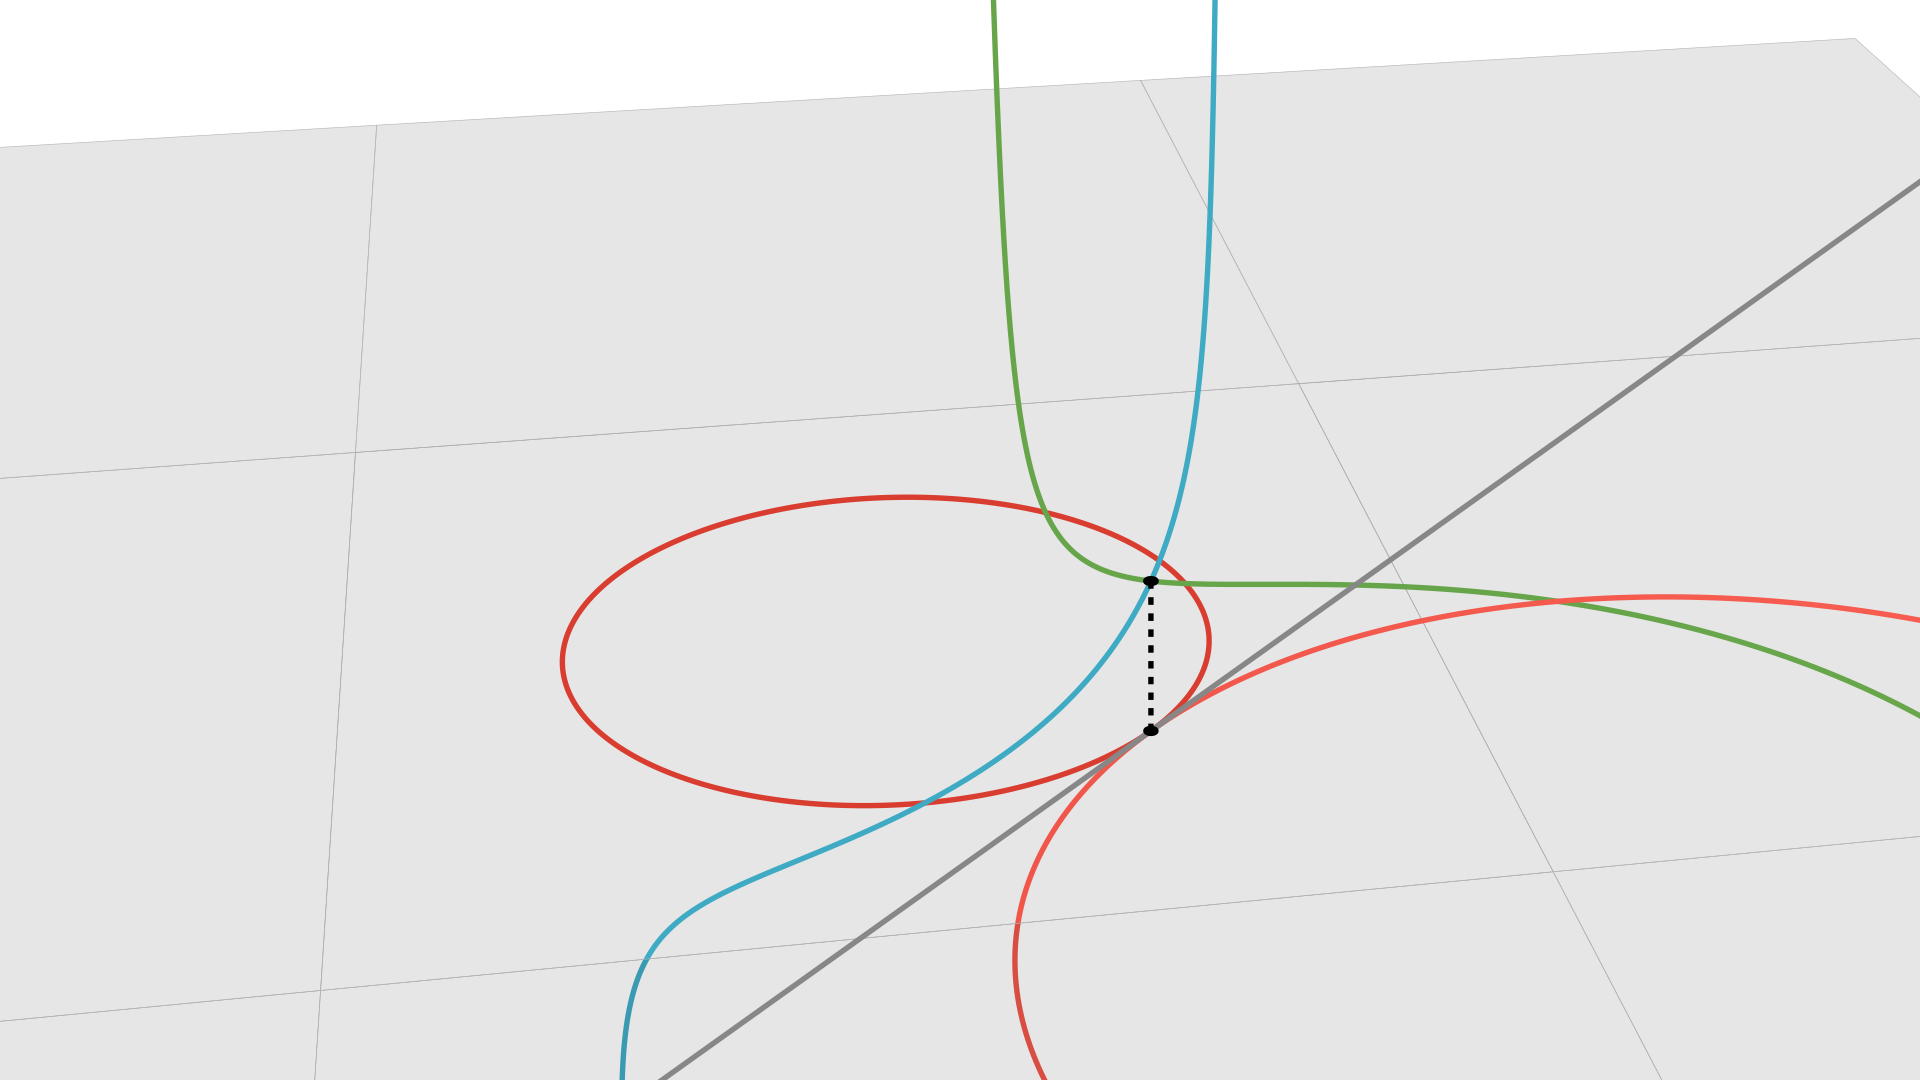
\includegraphics[width=0.8
    \textwidth, trim={5cm 0 4cm 2cm}, clip=true]{images/Diagram4b.png}
\end{figure}

Tangency problem in $\RR^2 \to $ Incidences problem in $\RR^3$.
}

\nfr{{Circle Tangencies: Tangencies to Incidences}

\begin{figure}[h]
    \centering
    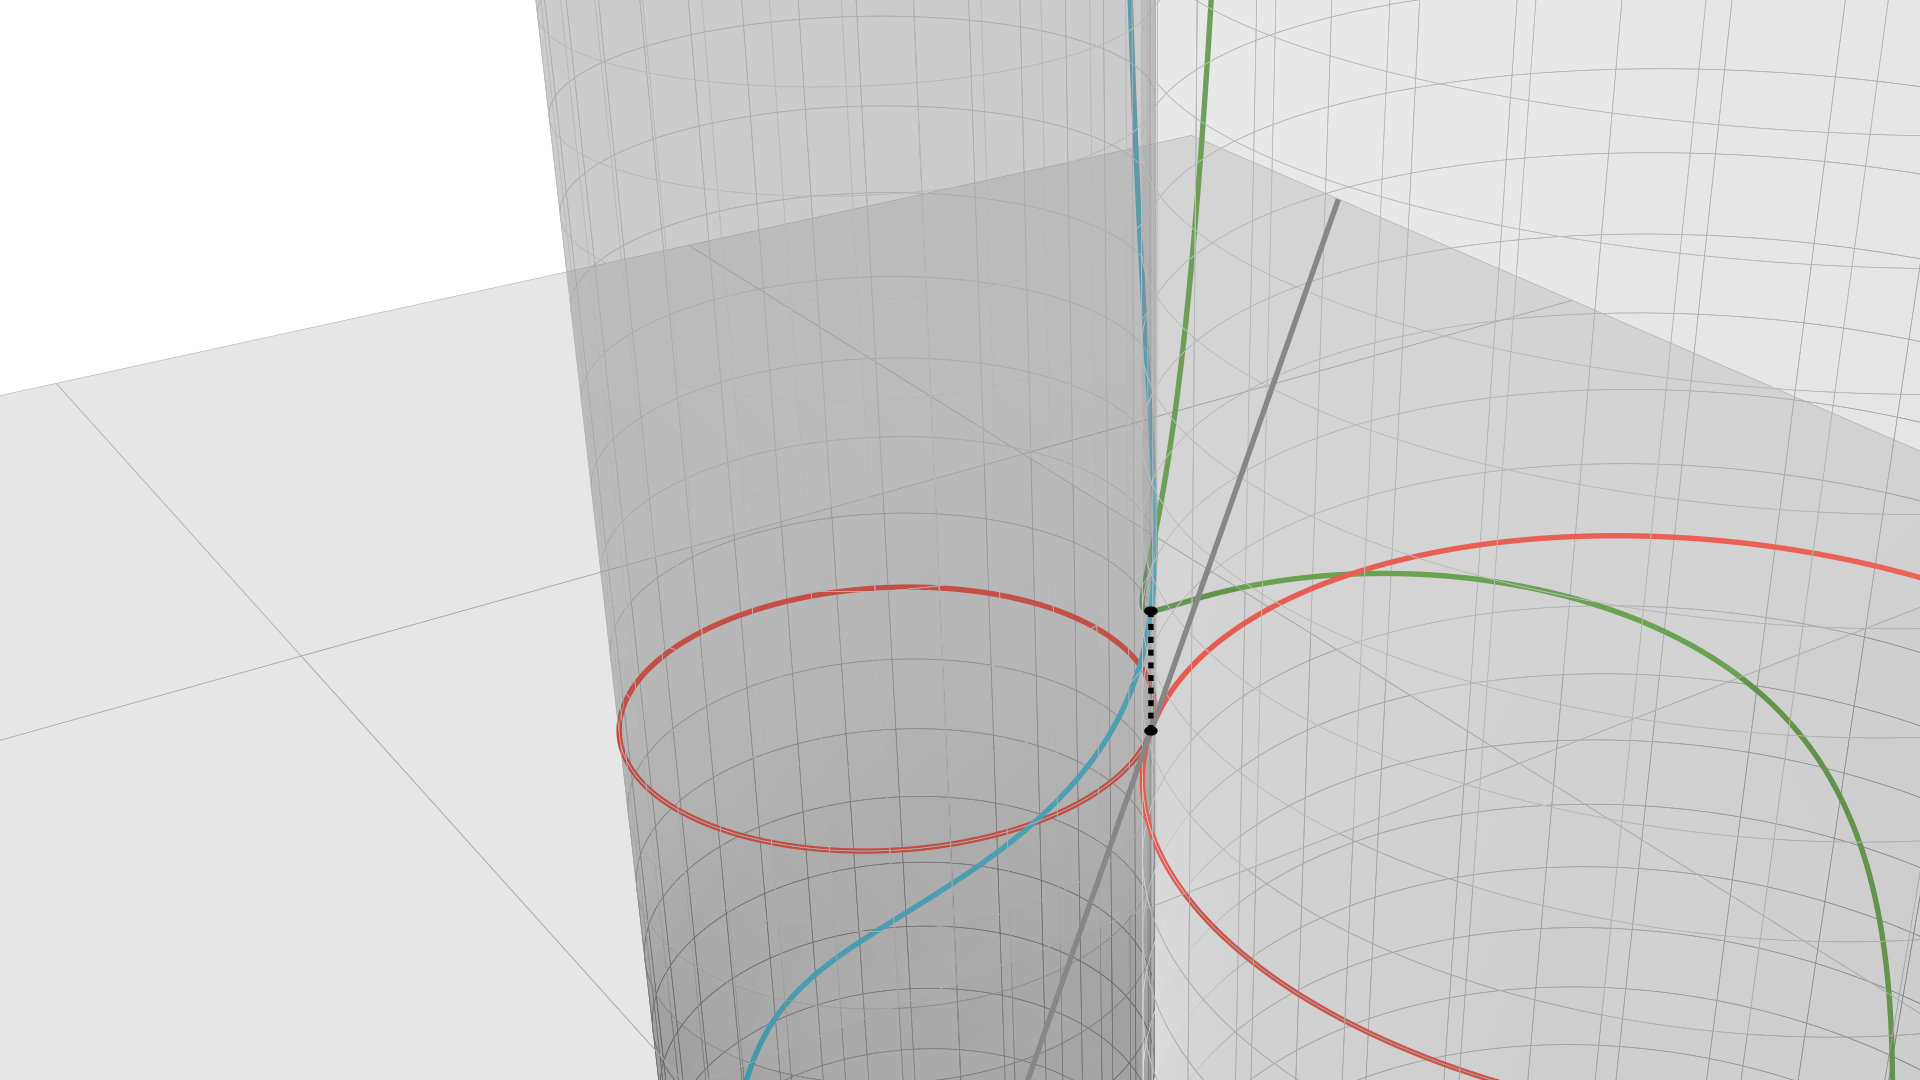
\includegraphics[width=0.8
    \textwidth, trim={5cm 0 4cm 2cm}, clip=true]{images/Diagram4c.png}
\end{figure}



Tangency problem in $\RR^2 \to $ Incidences problem in $\RR^3$.
}

\nfr{{Circle Tangencies: Tangent Vectors at Incidences}
Let us examine the tangent vectors at a point of incidence between two curves:
\begin{figure}[h]
    \centering
    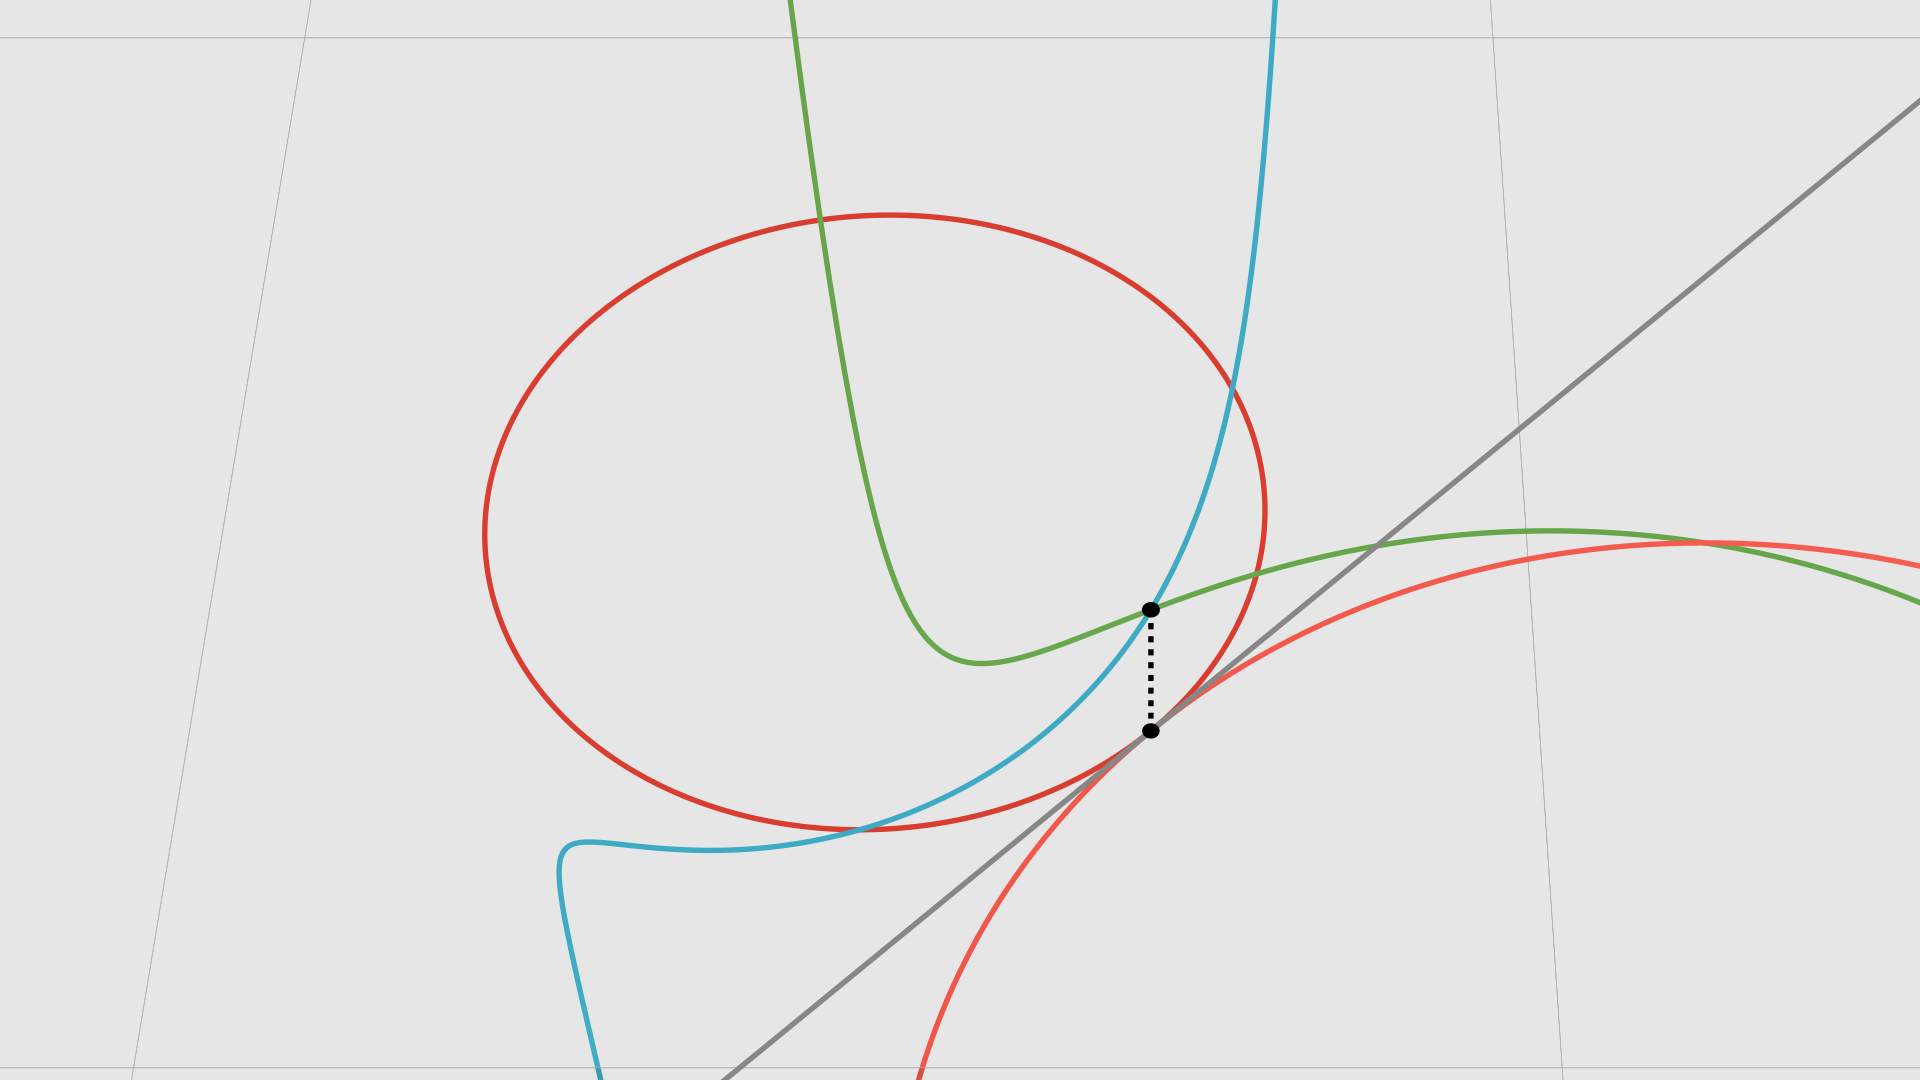
\includegraphics[width=0.8
    \textwidth, trim={5cm 0 4cm 2cm}, clip=true]{images/Diagram5a.png}
\end{figure}

}
\nfr{{Circle Tangencies: Tangent Vectors at Incidences}

\begin{figure}[h]
    \centering
    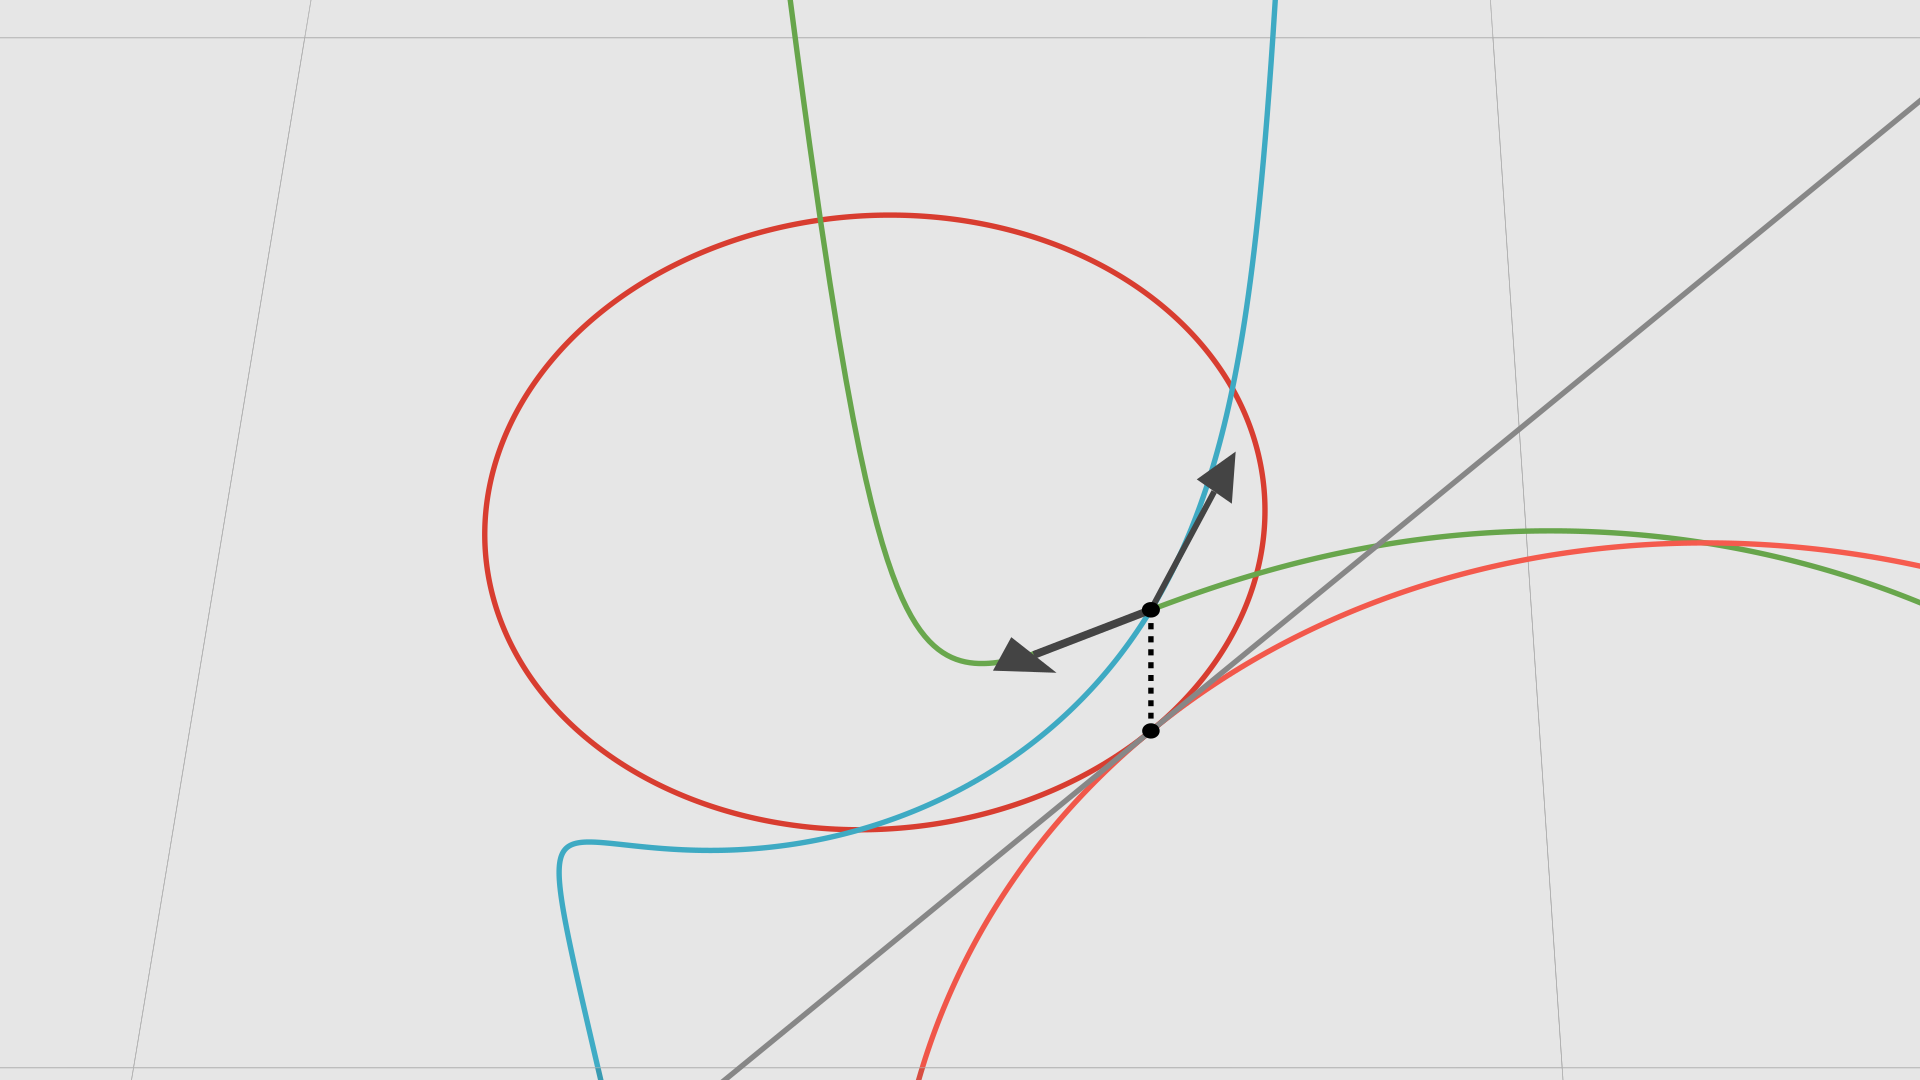
\includegraphics[width=0.8
    \textwidth, trim={5cm 0 4cm 2cm}, clip=true]{images/Diagram5b.png}
\end{figure} \pause
At every point of intersection, the tangent vectors span a vertical plane. 
}
\nfr{{Circle Tangencies: Tangent Vectors at Incidences}

\begin{figure}[h]
    \centering
    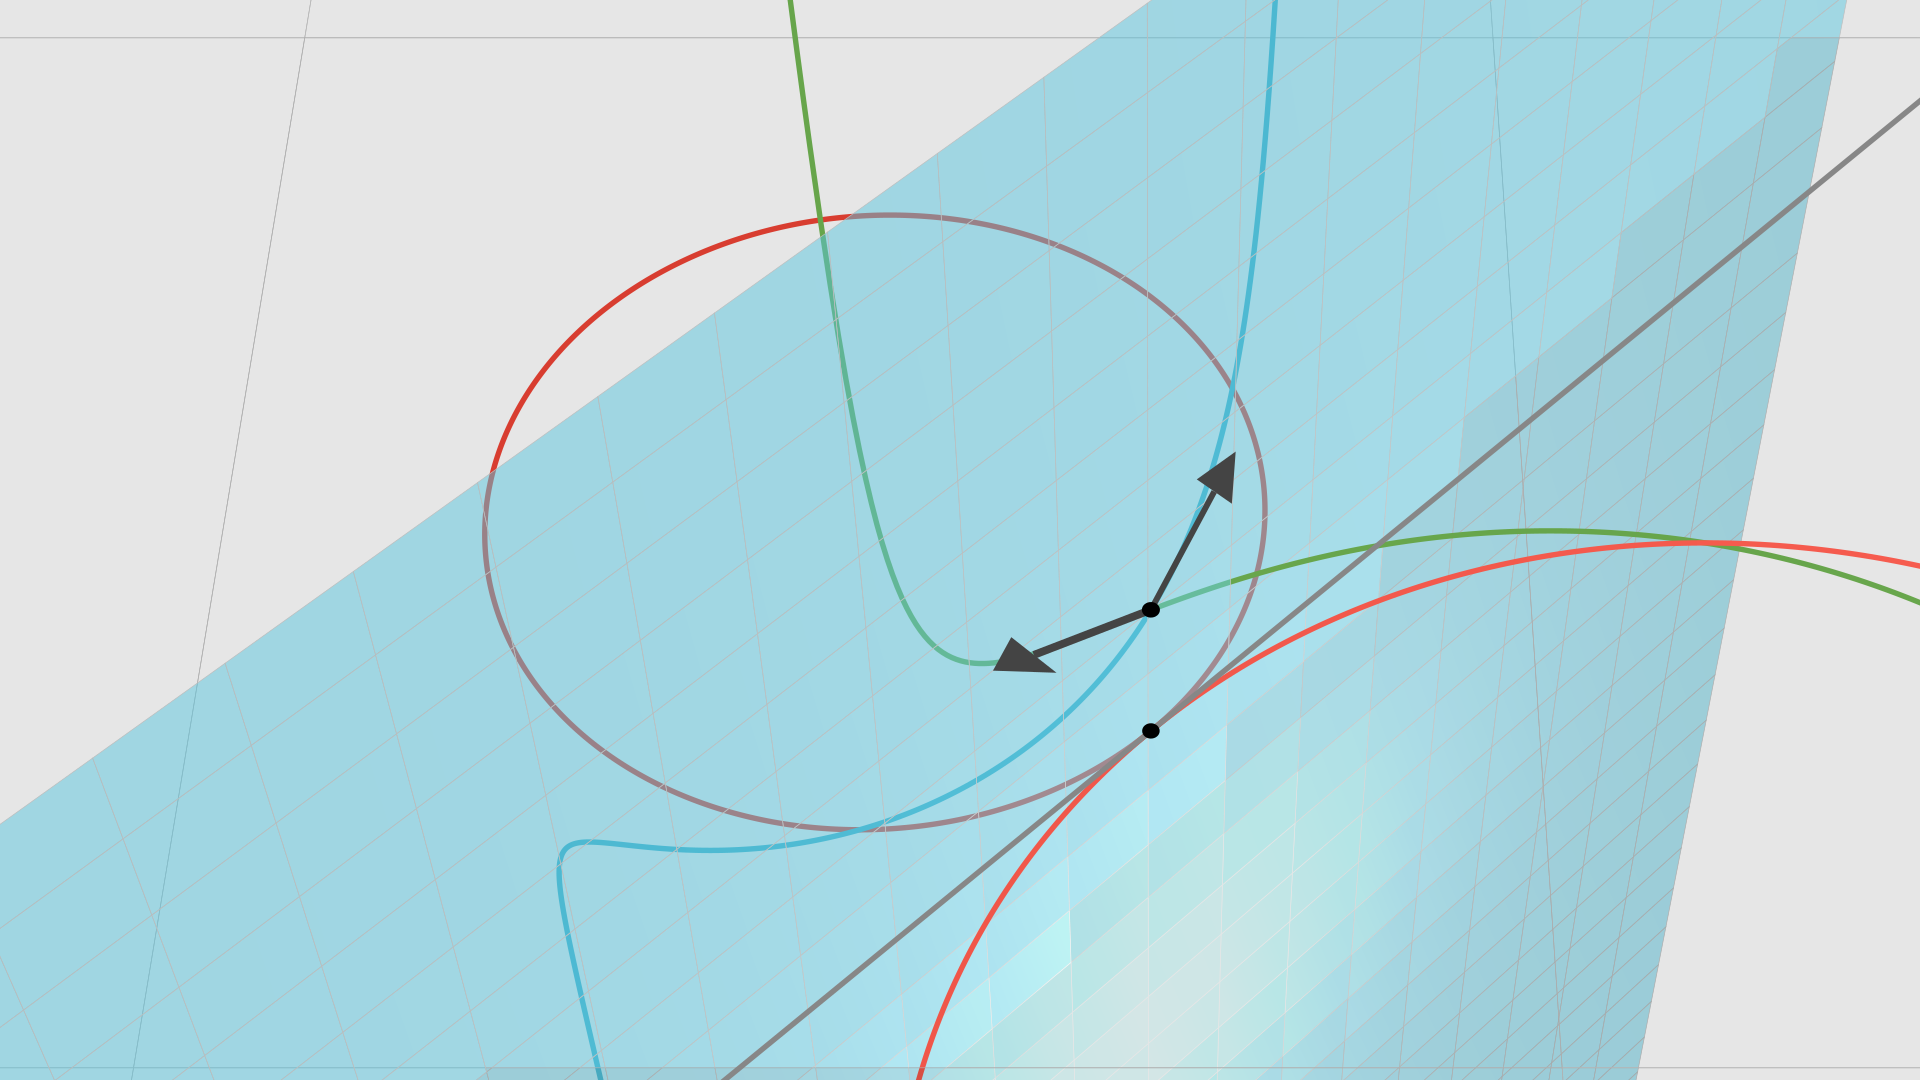
\includegraphics[width=0.8
    \textwidth, trim={5cm 0 4cm 2cm}, clip=true]{images/Diagram5c.png}
\end{figure}

At every point of intersection, the tangent vectors span a vertical plane. 

}



\nfr{{Circle Tangencies: Interpolation}
Let $P$ be a polynomial such that all $N^{3/2}$ incidences are contained in $Z(P)$. 

\begin{figure}[h]
    \centering
    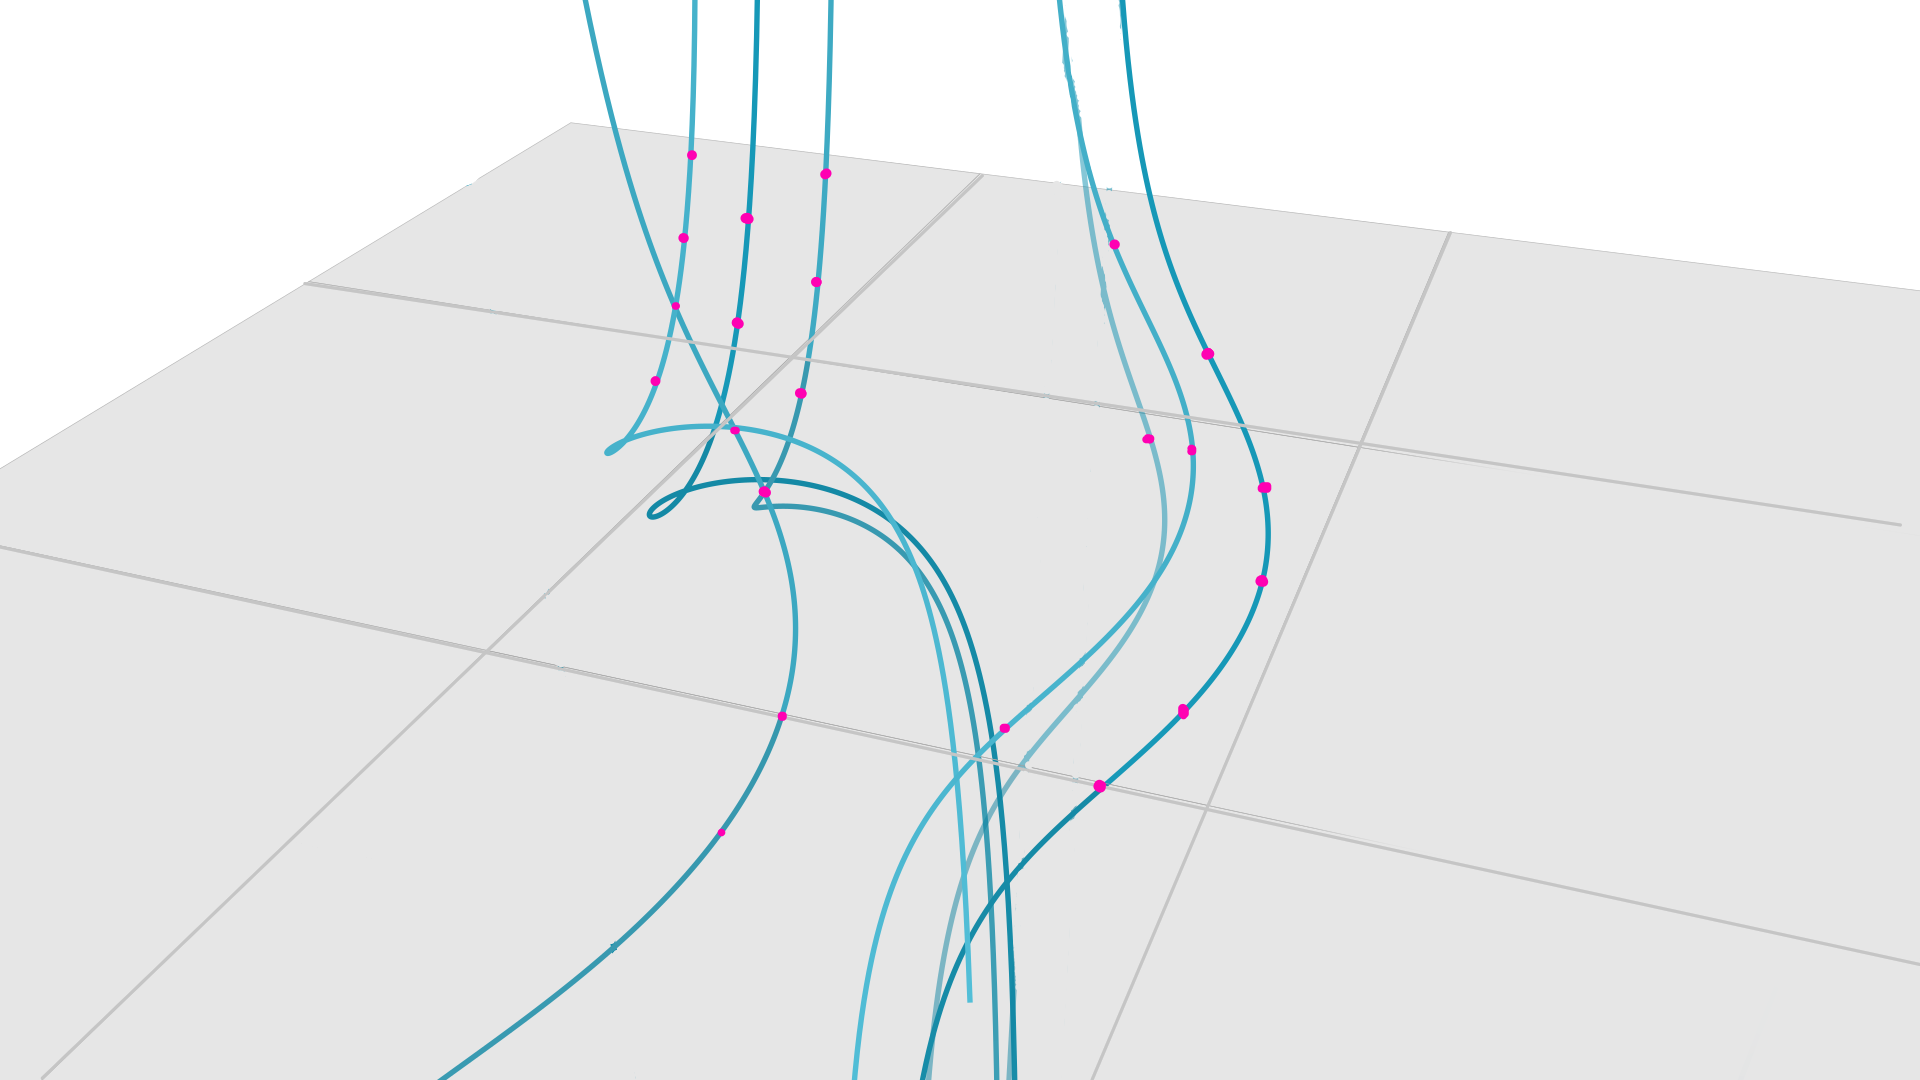
\includegraphics[width=0.7\textwidth]{images/lots_of_dots_a.png}
\end{figure}
}
\nfr{{Circle Tangencies: Interpolation}
Let $P$ be a polynomial such that all $N^{3/2}$ incidences are contained in $Z(P)$. 

\begin{figure}[h]
    \centering
    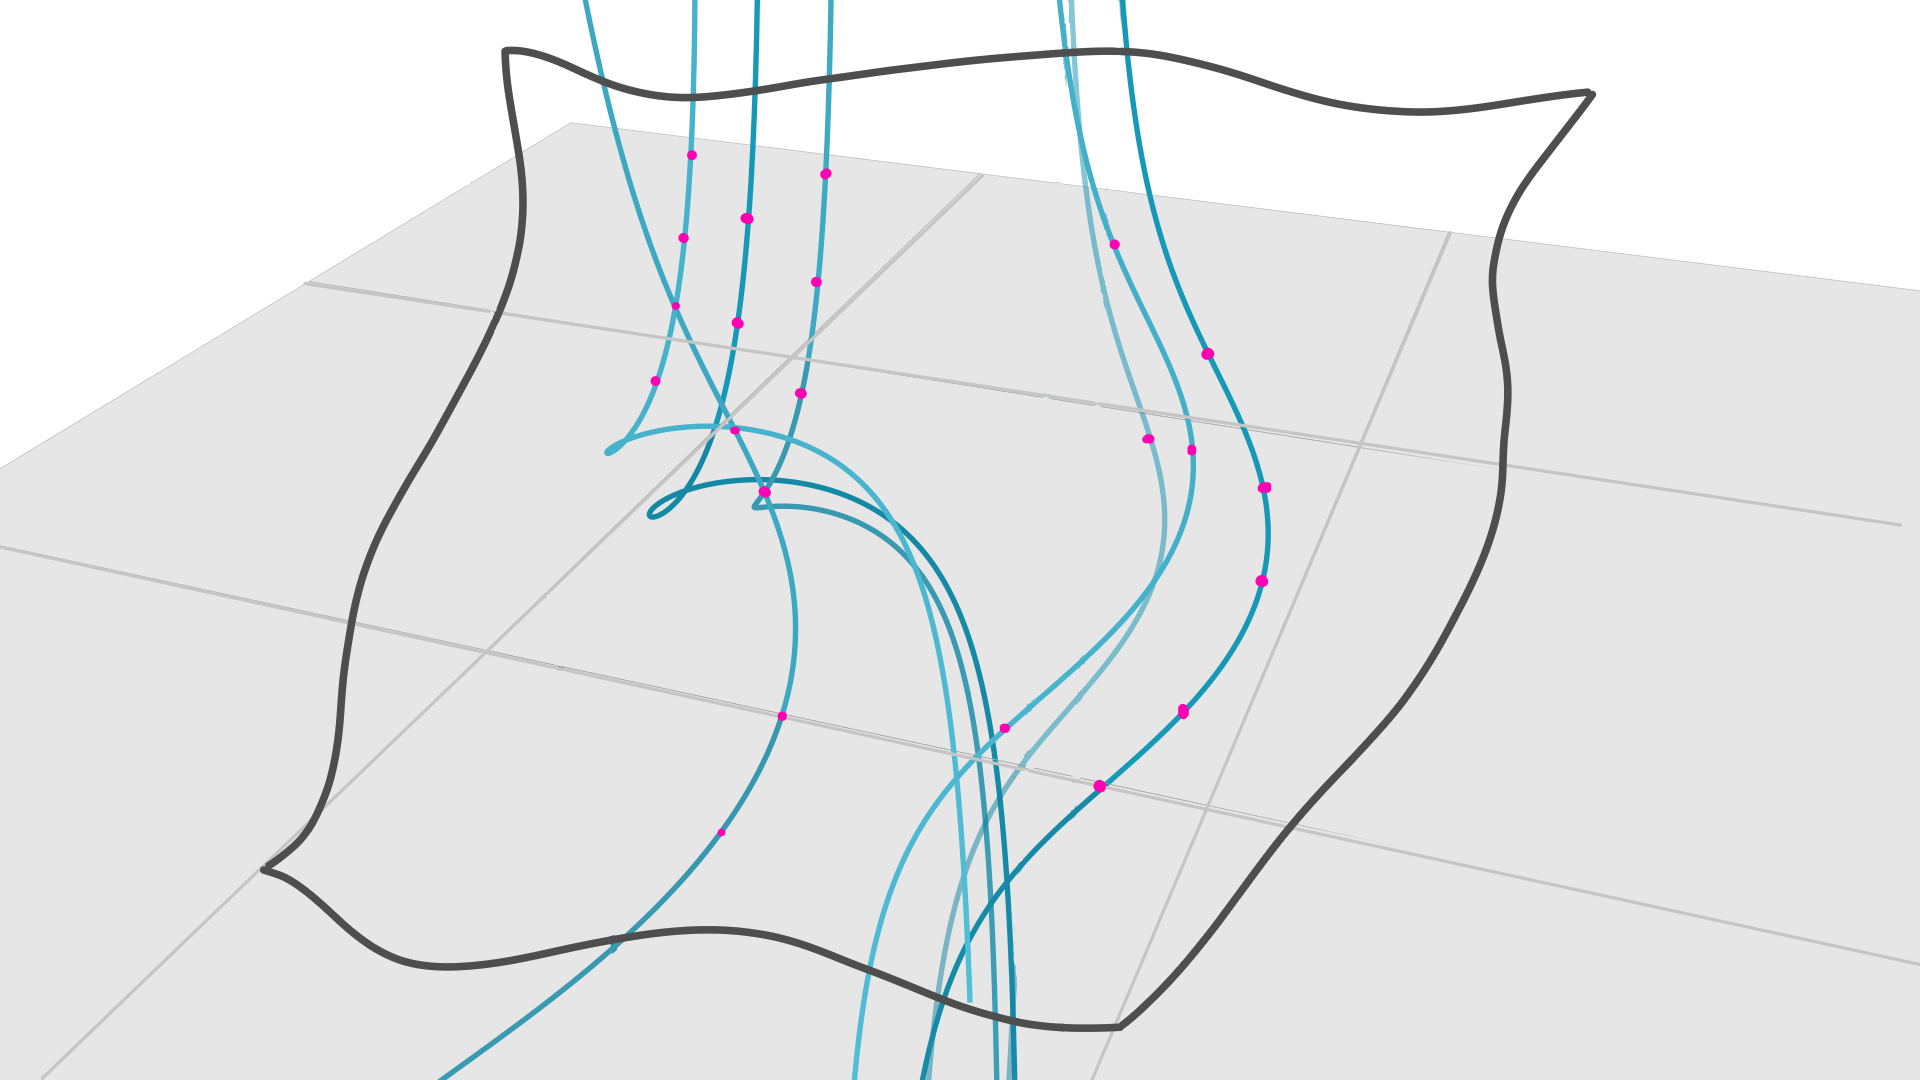
\includegraphics[width=0.7\textwidth]{images/lots_of_dots_b.png}
\end{figure}
}

\nfr{{Circle Tangencies: Interpolation}
Let $P$ be a polynomial such that all $N^{3/2}$ incidences are contained in $Z(P)$. 

\begin{figure}[h]
    \centering
    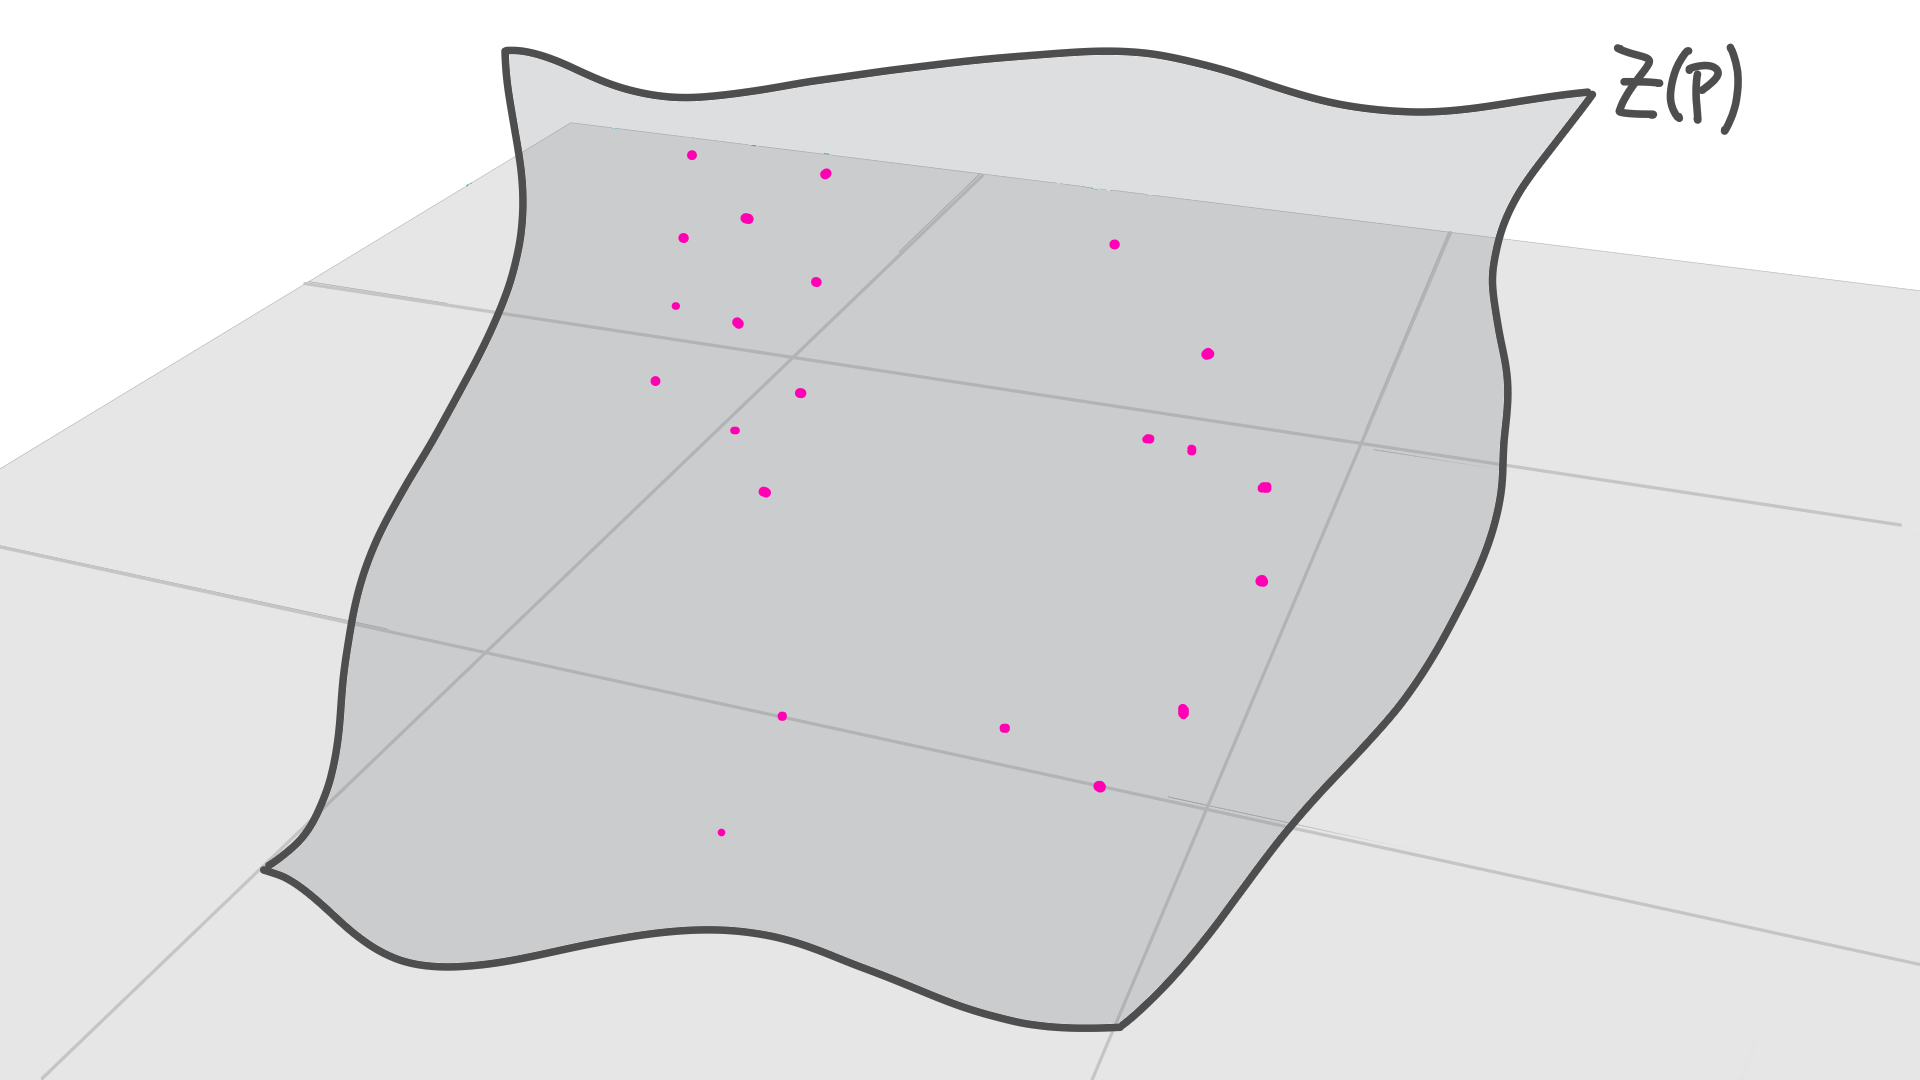
\includegraphics[width=0.7\textwidth]{images/lots_of_dots_c.png}
\end{figure}
}


\nfr{{Circle Tangencies: Interpolation}
Let $P$ be a polynomial such that all $N^{3/2}$ incidences are contained in $Z(P)$. 

\begin{figure}[h]
    \centering
    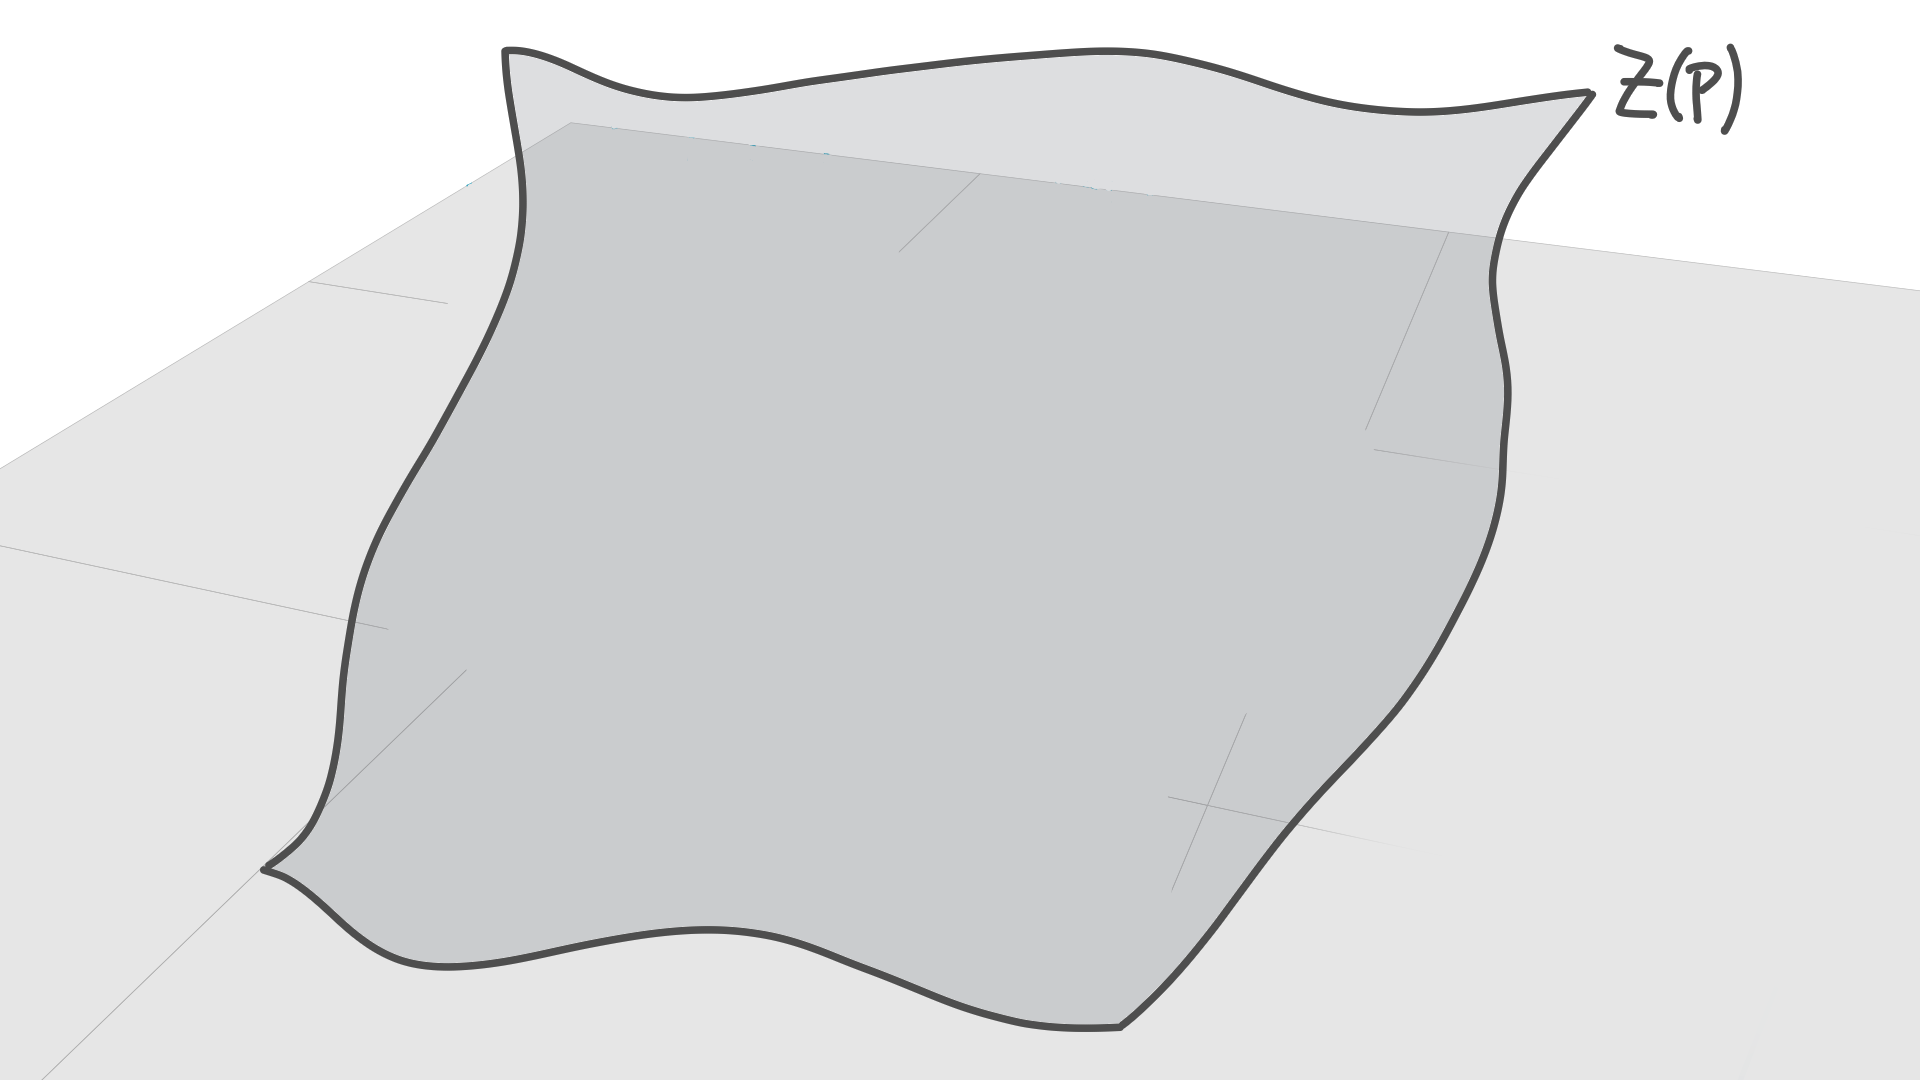
\includegraphics[width=0.7\textwidth]{images/lots_of_dots_d.png}
\end{figure}
\pause
\begin{itemize}
    \item Recall that $\dim \RR_{\deg \leq D} [X,Y,Z] \sim D^3$. \pause
    \item Each incidence point gives one linear equation for the coefficients. \pause
    \item $D^3 \sim N^{3/2} \implies D \sim N^{1/2}$.
\end{itemize}

}

\nfr{{Circle Tangencies: Interpolation}
\begin{figure}[h]
    \centering
    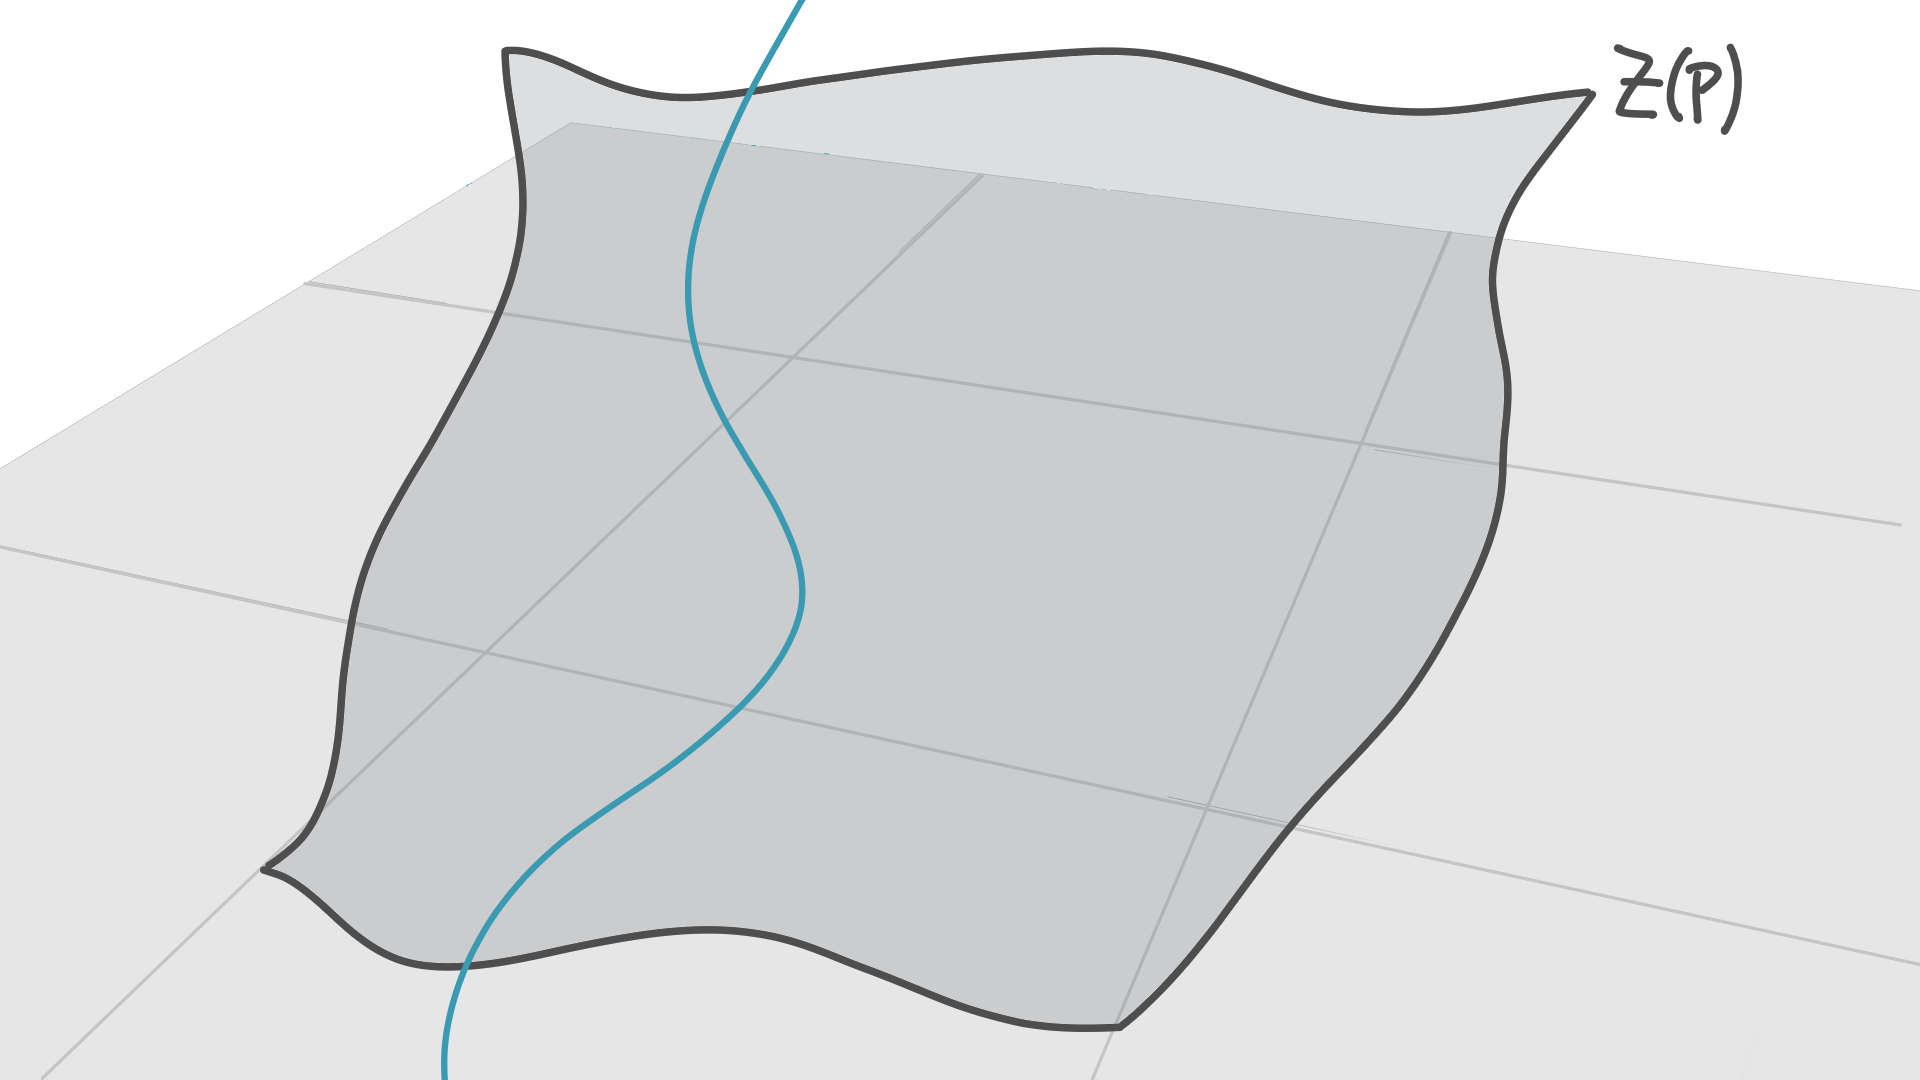
\includegraphics[width=0.7\textwidth]{images/lots_of_dots_e.png}
\end{figure}
}

\nfr{{Circle Tangencies: Interpolation}
\begin{figure}[h]
    \centering
    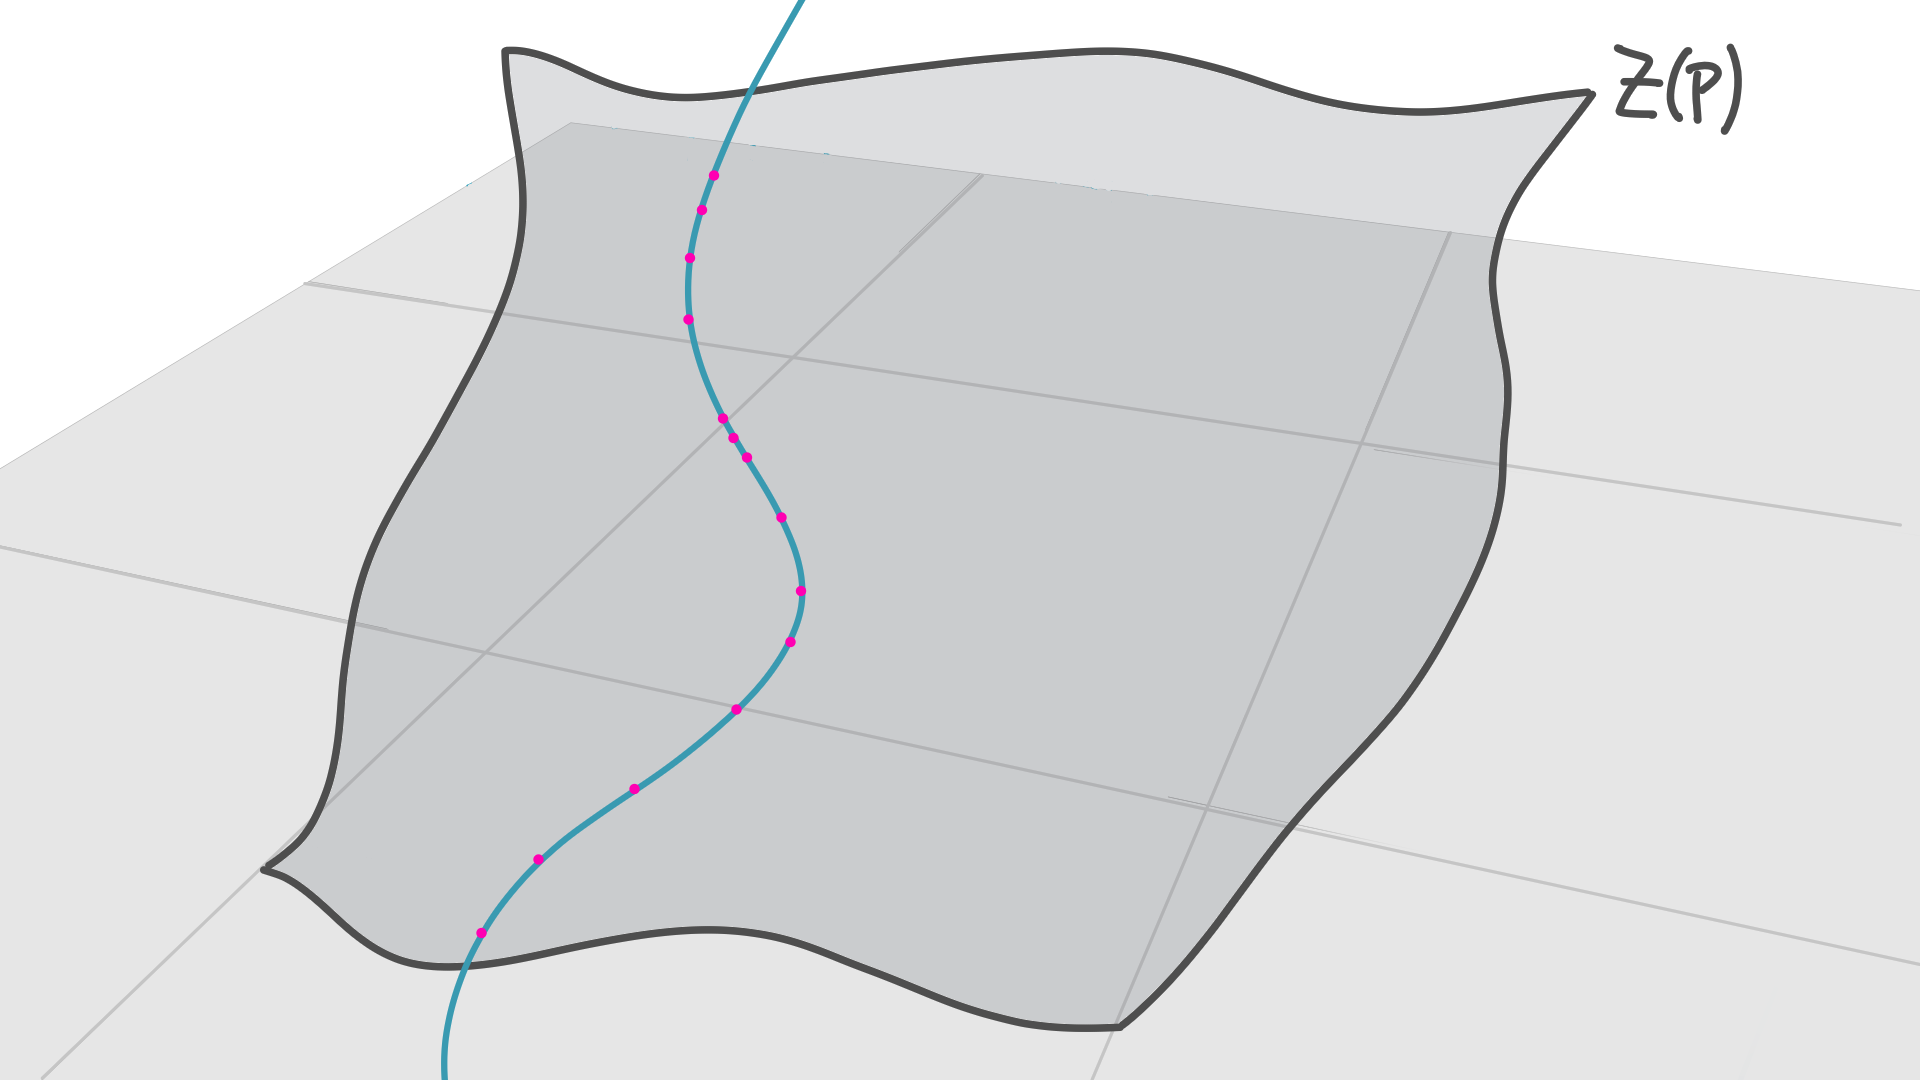
\includegraphics[width=0.7\textwidth]{images/lots_of_dots_f.png}
\end{figure}
\begin{itemize}
    \item Each curve $\beta(\gamma)$ contains $\gtrsim N^{1/2}$ points of intersection with $Z(P)$. \pause
    \item $\deg \beta(\gamma) = O (1)$ and $\deg P \sim N^{1/2}$ \pause
    \item $\implies \beta(\gamma) \subset Z(P)$ by Bézout's Theorem.
\end{itemize}
}

\nfr{{Circle Tangencies: Interpolation}
\begin{figure}[h]
    \centering
    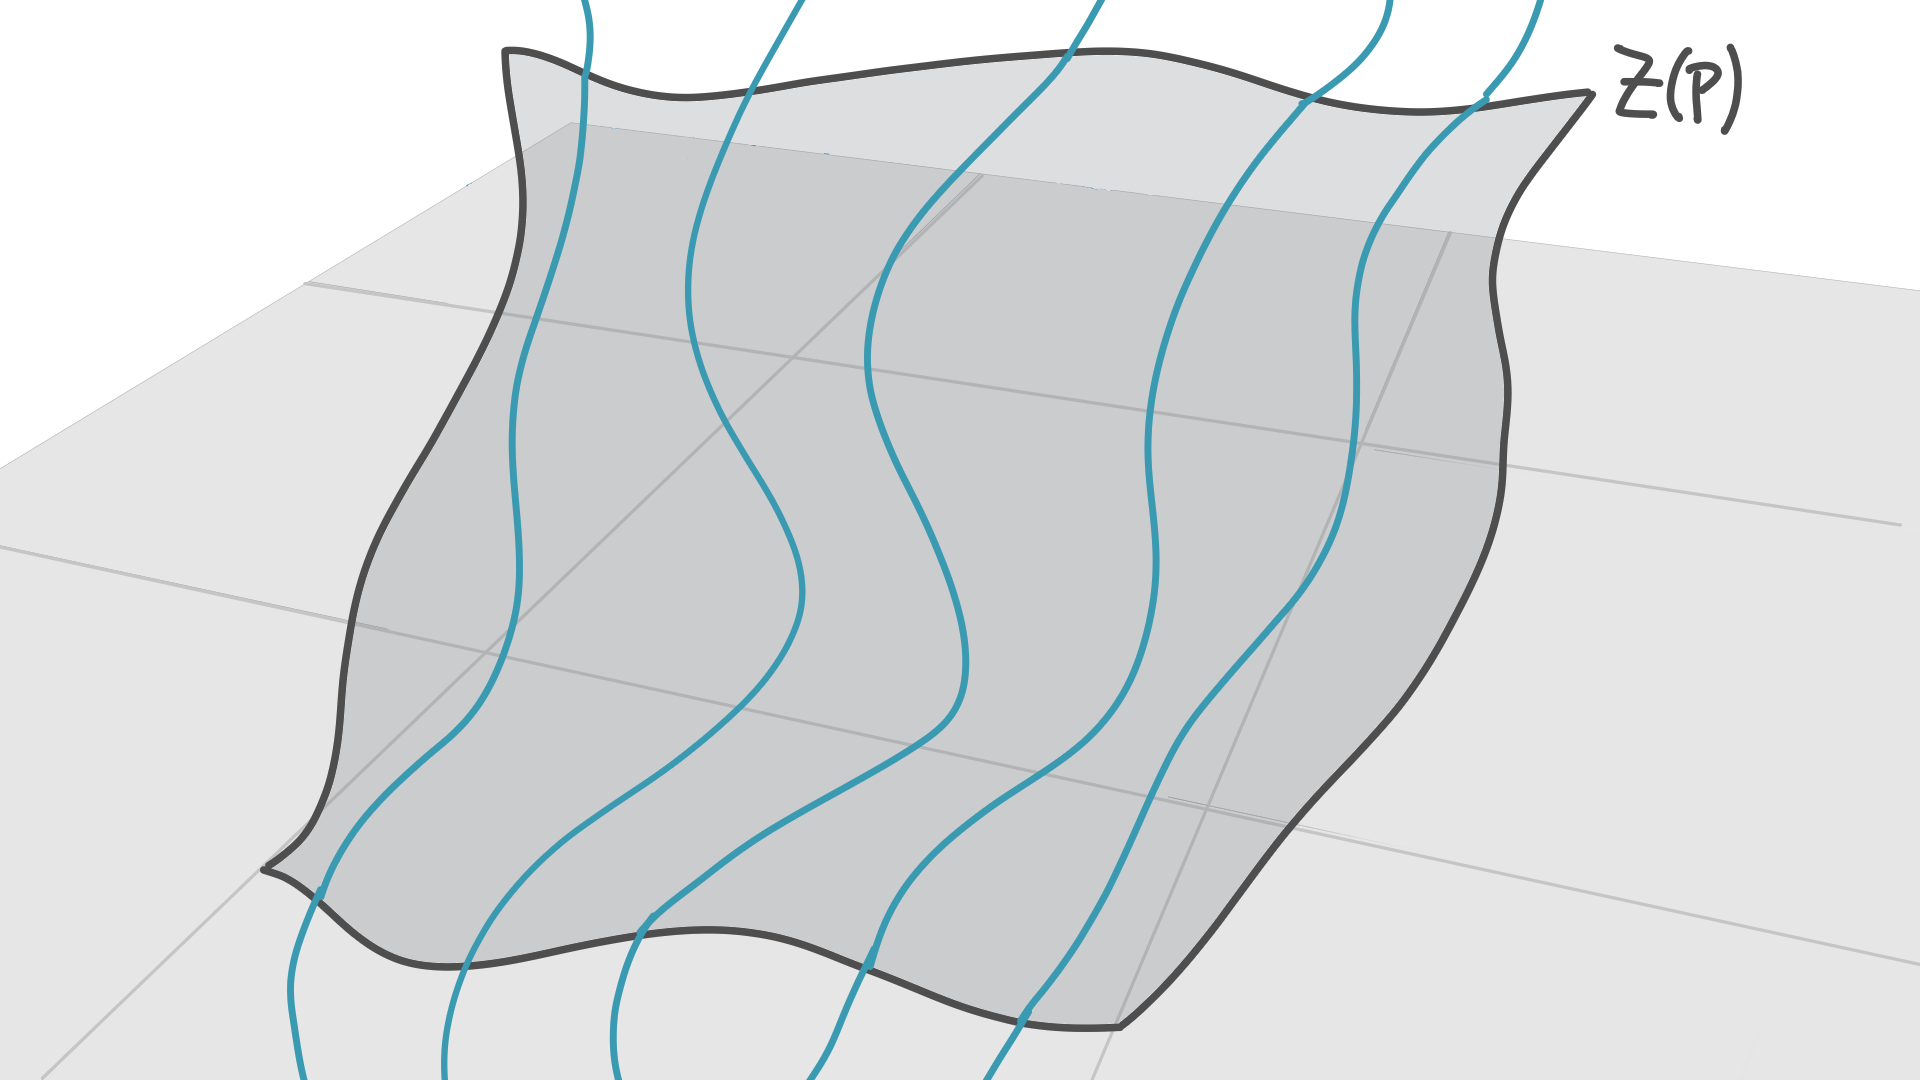
\includegraphics[width=0.7\textwidth]{images/lots_of_dots_g.png}
\end{figure}
\begin{itemize}
    \item Each curve $\beta(\gamma)$ contains $\gtrsim N^{1/2}$ points of intersection with $Z(P)$.
    \item $\deg \beta(\gamma) = O (1)$ and $\deg P \sim N^{1/2}$
    \item $\implies \beta(\gamma) \subset Z(P)$ by Bézout's Theorem.
\end{itemize}
}

\nfr{{Circle Tangencies: Interpolation}
\begin{figure}[h]
    \centering
    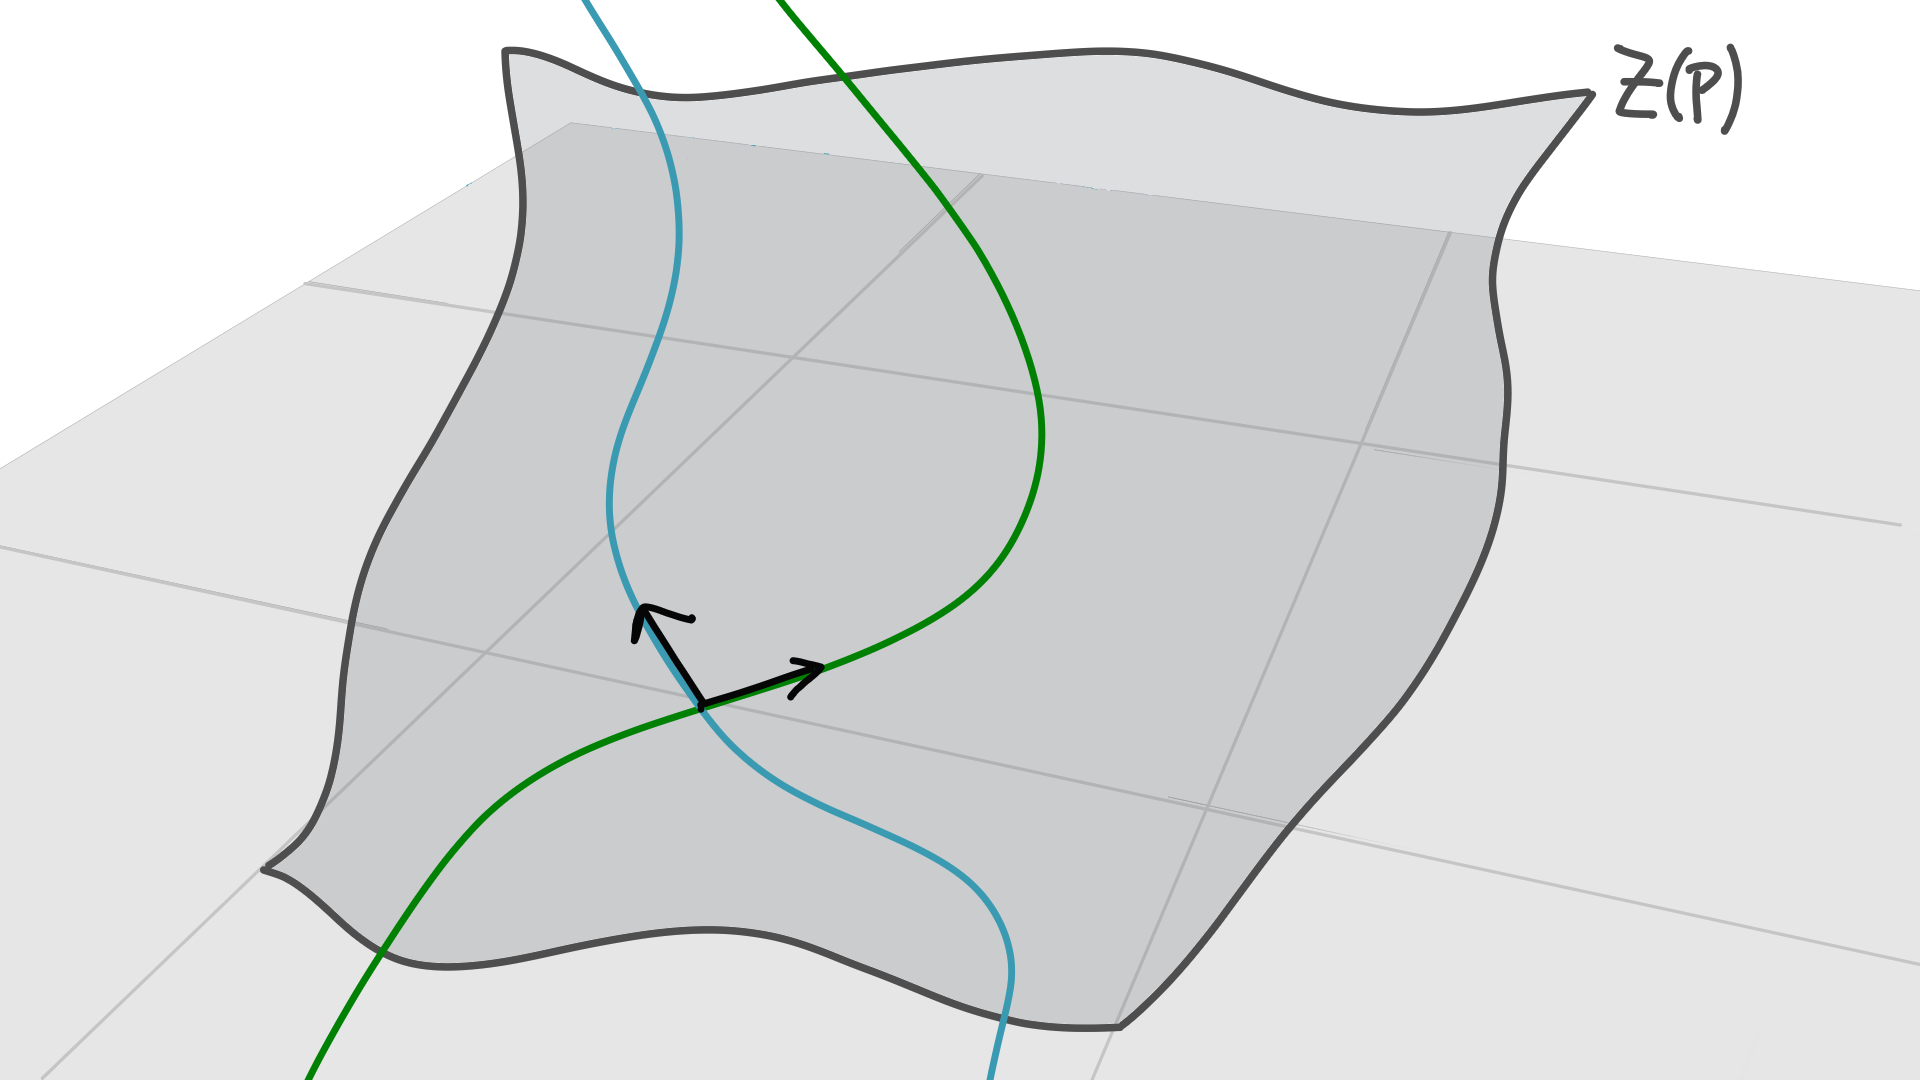
\includegraphics[width=0.7\textwidth]{images/lots_of_dots_h.png}
\end{figure}

}
\nfr{{Circle Tangencies: Interpolation}
\begin{figure}[h]
    \centering
    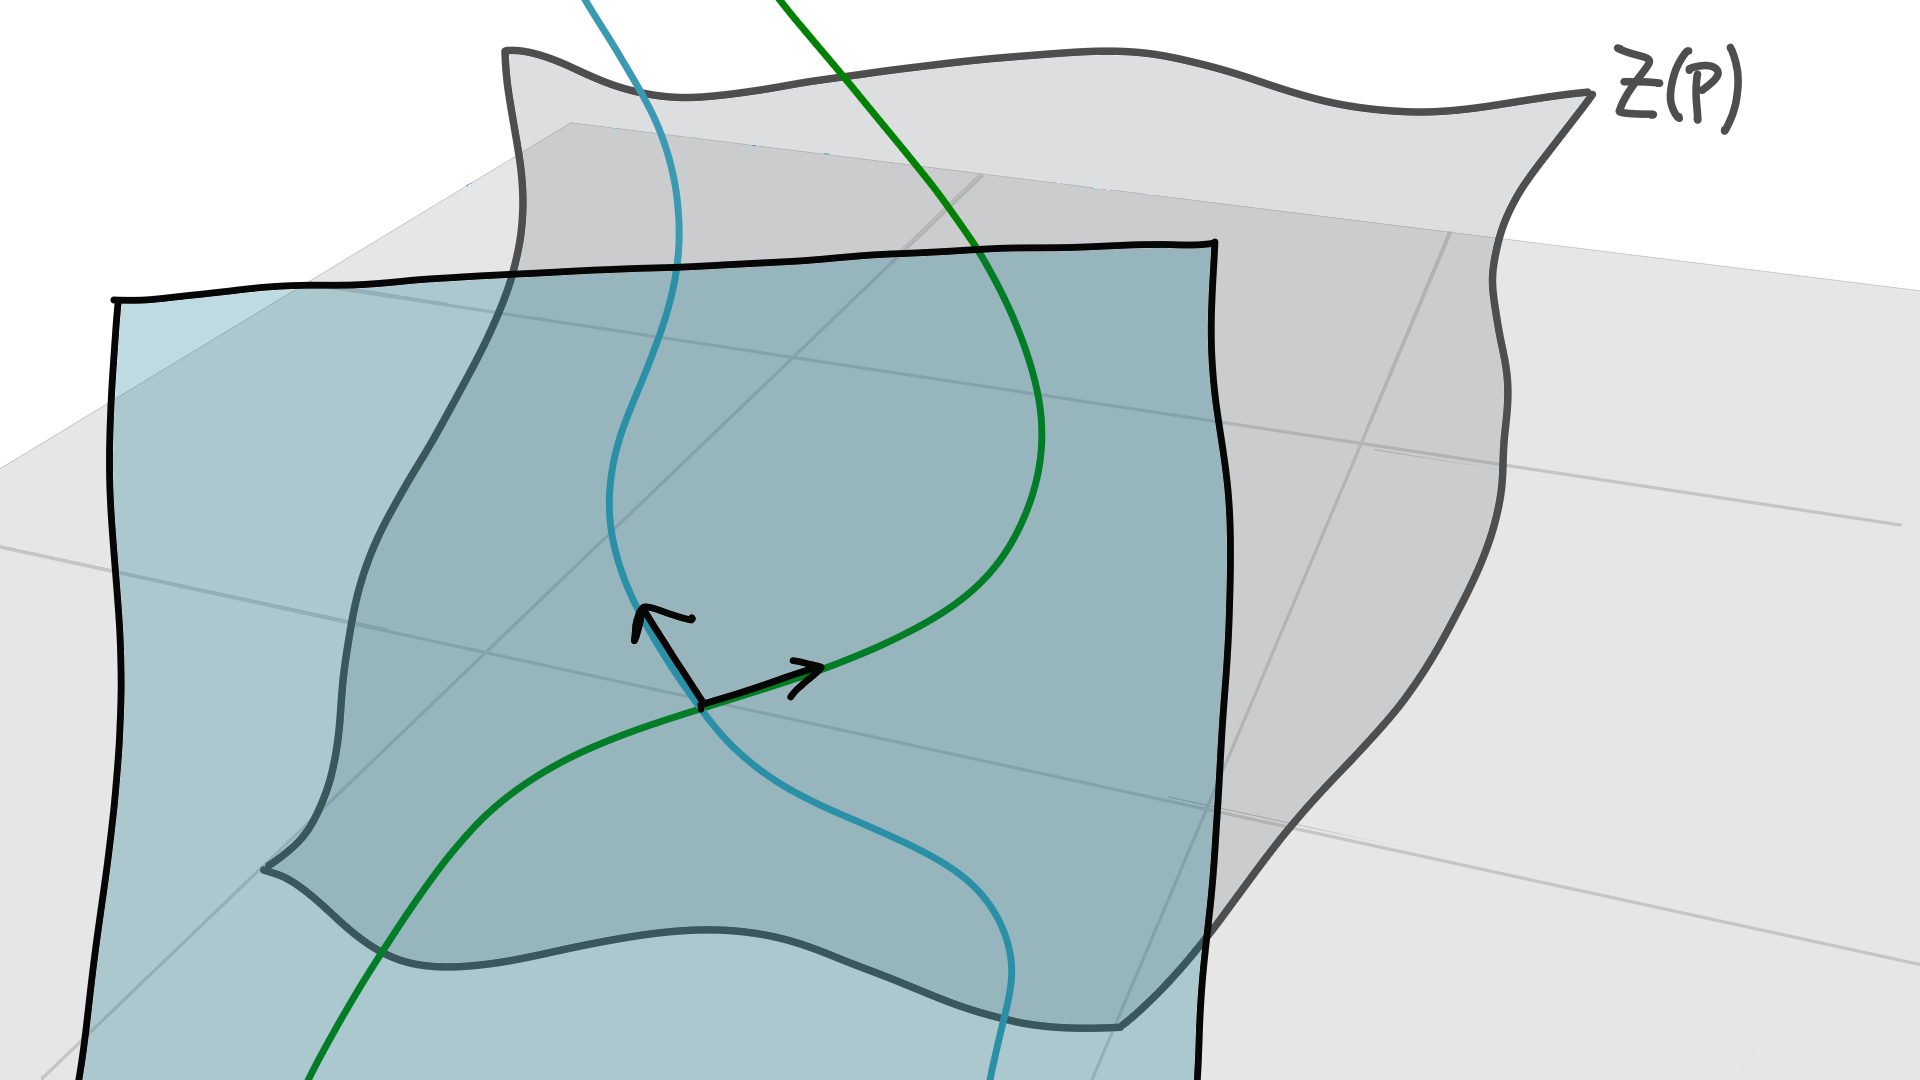
\includegraphics[width=0.7\textwidth]{images/lots_of_dots_i.png}
\end{figure}
\begin{itemize}
    \item Tangent vectors span the $z$-axis at tangencies, so $\partial_z P = 0$ on all incidences! 
    \item $\implies Z(\partial_z P)$ also contains all incidences. 
    \item $\implies P(X,Y,Z) = Q(X,Y)$.
\end{itemize}
}
\nfr{{Circle Tangencies: Interpolation}
\begin{figure}[h]
    \centering
    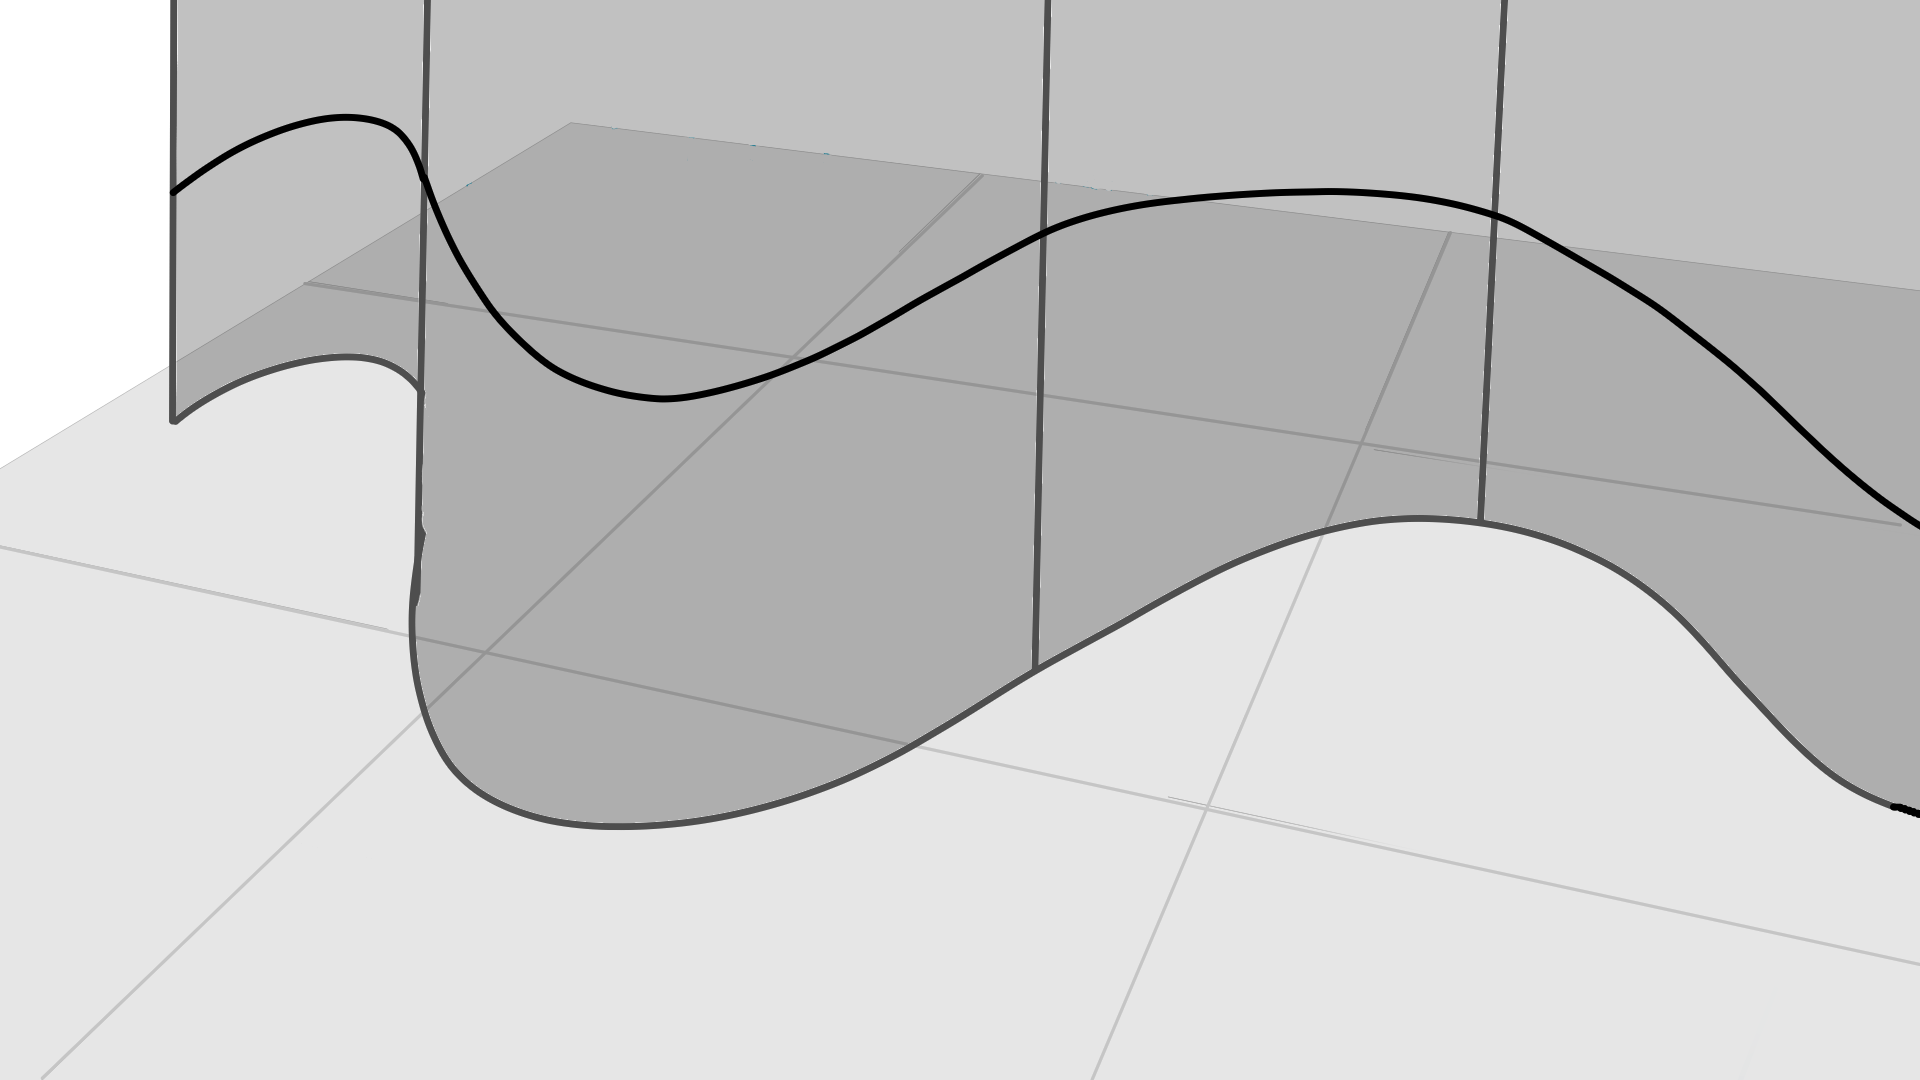
\includegraphics[width=0.7\textwidth]{images/lots_of_dots_j.png}
\end{figure}
$\deg Q \sim N^{1/2}$, but $Z(Q)$ contains $N$ circles.
Contradiction!
}
\nfr{{Circle Tangencies: Recap of Argument}
\begin{enumerate}
    \item Assume there are $\gtrsim N^{3/2}$ tangencies in our collection.
    \item Lift curves into $\RR^3$ and change into an incidence problem.
    \item Use a low degree polynomial $P$ to interpolate these points. (parameter-counting)
    \item Argue that if $Z(P)$ contains $\gtrsim N^{1/2}$ points of $\beta(\gamma)$ then $\beta(\gamma) \subset Z(P)$. (rigidity)
    \item Use structure of the objects to argue $P(X,Y,Z) = Q(X,Y)$
    \item Contradiction as degree of $Q$ is $N^{1/2}$ but contains $N$ circles.
\end{enumerate}
}

\bibliographystyle{unsrt}
\bibliography{slides}


\end{document}